% master.tex : master-fil for projektet
% ------------------------------------------------------------------------------
% Dette er hovedfilen for projektet, hvori indhold fra alle input-filer (tekst,
% billeder, litteraturdatabaser, osv.) samles

% Dokumenttypen 'book' er valgt pga. dens mange fleksible indstillinger
% Se https://tex.stackexchange.com/a/36989/118167
\documentclass[11pt,a4paper,twoside,openright,danish]{book}

% Variabler, som bruges til automatisk at indsætte titel, forfattere, osv. på
% forsiden og titelbladet.
\def \projecttitle       {Optimering}
\def \projectsubtitle    {Lineær programmering}
\def \projecttheme       {Simplex}
\def \projectdegree      {Matematik}  % eller Matematik-Økonomi/Teknologi
\def \projectperiod      {Forårssemesteret 2020}
\def \projectnumber      {P2}
\def \projectgroup       {B305}
\def \projectauthors     {
  Caroline Nørskov Budsted Weje\\
  Henriette Høiberg Bjørn\\
  Jesper Soelberg Jensen\\
  Jonas Winther\\
  Katharina Bramsing Bach\\
  Mie Frederiksen Larsen
  % ...
}
\def \projectsupervisors {
  Projektvejleder 1\\
  Projektvejleder 2
  % ...
}

% Preamblet indeholder alle de indstillinger og makroer, som skal indsættes for
% hovedindholdet, og i denne skabelon samles det i filen aaumath.sty, som
% definerer en pakke, der kan indlæses med \usepackage.
\usepackage{aaumath}
\setlength{\parindent}{0cm}

% Dokumentets indhold indsættes mellem \begin- og \end-makroerne for
% 'document'-blokken
\begin{document}

% Dokumentets 'front matter' tælles ikke med ifm. antal sider og nummereres med
% romerske tal. Herunder hører f.eks. forsiden, titelbladet, forordet og
% indholdsfortegnelsen.
\frontmatter
% incl/misc/frontpage.tex : rapportens forside
% ------------------------------------------------------------------------------


\backgroundsetup{
  scale = 1,
  angle=0,
  opacity=1,
  contents = {
    
\includegraphics[width=\paperwidth,height=\paperheight]{fig/img/aau/waves.pdf}
  }
}
\BgThispage
\pdfbookmark[0]{Forside}{forside}
\begin{titlepage}
  \centering
  \phantom{}
  \vspace{2cm}

  % AAU-segl
  \begin{minipage}[c]{0.2\paperwidth}
    \centering
    \makebox[0pt]{
      % fig/tikz/aau-badge.tex : AAU-logo til forsiden
% ------------------------------------------------------------------------------

\begin{tikzpicture}
  % Tegn hvid cirkel og tilføj det gennemsigtige, blå logo ovenpå
  \node[circle,color=white,fill=white,minimum size=1.175\textwidth] at (0,0) {};
  \node at (0,0) {
\includegraphics[width=\textwidth]{fig/img/aau/logo-circle.pdf}};
\end{tikzpicture}

    }
  \end{minipage}

  % Hovedindhold
  \vspace{4cm}
  {\fontfamily{bch}\selectfont
    \fboxsep0pt\colorbox{white}{
      \begin{minipage}{\textwidth}
        \centering
        \color{AAUblue1}

        \vspace{2em}
        {\Huge\bfseries\projecttitle}

        {\Large\bfseries\projectsubtitle}

        \bigskip
        \parbox{\textwidth}{\centering\large\projectauthors}

        \bigskip
        {\bfseries\large{\projectnumber}-Projekt, Gruppe \projectgroup, \projectdegree}
        \vspace{2em}
      \end{minipage}
    }
  }

\end{titlepage}

% incl/misc/titlepage.tex : rapportens titelblad
% ------------------------------------------------------------------------------
% Titelbladet genereres af makroen \aautitlepage, som er defineret i
% /incl/pre/ext/aautitlepage.sty


\pdfbookmark[0]{Titelblad}{titelblad}
\aautitlepage{
  \projectinfo{
    \projecttitle
  }{
    \projecttheme
  }{
    \projectperiod
  }{
    Gruppe \projectgroup
  }{
    \parbox[t]{\textwidth}{\projectauthors}
  }{
    \parbox[t]{\textwidth}{\projectsupervisors}
  }{
    \today
  }
}{
  \textbf{Institut for Matematiske Fag}\\
  Skjernvej 4A\\
  DK-9220 Aalborg Ø\\
  \href{http://math.aau.dk}{http://math.aau.dk}
}{
  % incl/misc/abstract.tex : projektets abstract
% ------------------------------------------------------------------------------
% Et abstract er et kort resume af rapporten, som vises på titelbladet

Linear programming is used to optimize linear programming problems. In this project, different methods for solving linear programming problems. One method explored is the geometric method, in which the level sets are used to find the solution to the problem. The other method is the simplex method. Here, the geometric property of the simplex method is explored and used to deduce the simplex method. The simplex method uses linear algebra to jump between basic solutions, to find the optimal one. This is implemented by the full tabular method, the lexiographic rule and the big M-method. The big M-method is used to solve organizational problems. The found methods are then used, to solve a case about a company wanting to optimize their expenses to salary. 
}

% incl/misc/contents.tex :
% ------------------------------------------------------------------------------

\pdfbookmark[0]{Indhold}{indhold}

% Indstillingerne i denne fil er grupperet, så de ikke påvirker andre dele
\begingroup

% Slå twoside fra midlertidigt for at undgår sideskift
\makeatletter
\@twosidefalse
\makeatother

% Placer indholdsfortegnelsen på sin egen side (bedst når den kun fylder en side)
\tableofcontents
\clearpage

% Placer oversigtslisterne på efterfølgende sider
\let\clearpage\relax
\listoffigures
\lstlistofpro
\lstlistofalg

\endgroup


% Dokumentets 'main matter' (hovedindhold) er der, hvor det meste indhold skal
% sættes ind. Sider og overskrifter er nummererede med arabiske tal.
\mainmatter

% Input-filer bør opdeles således, at hver fil svarer til et kapitel. Makroen
% \include indsætter et sideskift og indholdet fra den givne stil.

\chapter{Reminders}

forkortelser for sætninger korrolarer osv.
\begin{table}[h]
\begin{tabular}{|l|l|}
stn & sætning \\
lma & Lemma \\
prop & proposition \\
defn & definition \\
kor & korrolar \\
eks & eksempel \\
alg & algoritme
\end{tabular}
\end{table}
\chapter{indledning}

\chapter{Problemanalyse}
\section{problemformulering}
\chapter{Lineær algebra}
Dette kapitel er skrevet med udgangspunkt i 

Lineær algebra bruges til at løse lineære ligningssystemer. 
En af de mest nyttige algoritmer, til at løse sådanne ligningssystemer, er Gaussisk elimination, som vil blive beskrevet senere i dette kapitel.

\section{Matricer}
Lineære ligningssystemer kan opskrives i matricer. 
En matrix er defineret i Definition \ref{def:matricer}.

\begin{defn} [Matrix]\label{def:matricer}
En matrix er en rektangulær tabel over skalarer. 
Størrelsen på en matrix er $m \times n$, hvor $m$ er antal rækker og $n$ er antal søjler. 
En matrix kaldes kvadratisk hvis $m=n$. 
Skalaren i den $i$'te række og $j$'te søjle kaldes $(i,j)$-indgangen.
\end{defn}

Herunder ses en matrix $\underset{m \times n}{A}$ og dens indgange, $a_{i,j}$. Den $i$'te række i A betenges $\vec{a}_i$, mens den $j$'te søjle angives $\vec{A}_j$.

\begin{align*}
\underset{m \times n}{A} = \begin{bmatrix}
	a_{1,1} & a_{1,2} & \dots & a_{1,j} & \dots & a_{1,n} \\
	a_{2,1} & \ddots  &       &         &       & \vdots \\
	\vdots  &         & \ddots &        &       & \vdots \\
	a_{i,1} &         &       & a_{i,j} &       & \vdots \\
	\vdots  &         &       &         & \ddots& \vdots \\
	a_{m,1} & \dots   & \dots & \dots   & \dots & a_{m,n} 
\end{bmatrix}
\end{align*}

Matricer kan bruges til at vise mange forskellige ting fra den virkelige verden, det kan være antal af varer solgt fra forskellige butikker, eller prisen på forskellige produkter. 

\begin{eks}
Herunder ses en $4 \times 3$-matrix, der viser antallet af solgte varer fra tre forskellige butikker. Hver række i matricen repræsenterer en bestemt vare, mens hver søjle repræsenterer en butik. Den første række viser altså hvor mange trøjer hver butik har solgt.
\begin{align*}
\begin{matrix}
	Trøjer \\
	Kjoler \\
	Bukser \\
	Jakker
\end{matrix}
\begin{bmatrix}
	24 & 35 & 43 \\
	10 & 47 & 24 \\
	33 & 25 & 32 \\
	28 & 51 & 37
\end{bmatrix}
\end{align*}
I denne matrice kan man se, at der i dens $(2,3)$-indgang står $24$, hvilket betyder, at den tredje butik har solgt $24$ kjoler. Der står i dens $(3,1)$-indgang $33$, hvilket betyder, at den første butik har solgt $33$ par bukser.
\end{eks}

\begin{defn}[Transponeret matrix]
Lad $A$ være en $m \times n$ matrix. Så er den transponerede matrix, $A^T$, en $n \times n$ matrix, hvor hver indgang i $A^T$, $(i,j)$ er den $(j,i)$'te indgang i $A$
\label{def:(transmatrix)} 
\end{defn}
Det vil sige at rækkerne i $A$, bliver til søjlerne i $A^T$. Og søjlerne i $A$ bliver til rækkerne i $A^T$.

\begin{eks}
Givet en matrix $A$ 	bestemmes nu den transponerede
\begin{align*}
A = \begin{bmatrix}
	5 & 3 & 3 \\
	1 & 2 & 5
\end{bmatrix}
\end{align*}

\begin{align*}
A^T = \begin{bmatrix}
	5 & 1  \\
	3 & 2  \\
	3 & 5
\end{bmatrix}
\end{align*}
Det ses at $A$ er en $2 \times 3$ matrix og $A^T$ er en $3 \times 2$ matrix. 
\end{eks}


En bestemt type af matrix er en identitetsmatrix, der betegnes $I_n$. 

\begin{defn} [Identitetsmatrix]\label{def:imatrix}
For hvert positivt heltal $n$, er $n \times n$ identitetsmatricen, $I_n$, den $n \times n$ matrix, hvor hver søjle er standardvektorerne $\vec{e_1}$, $\vec{e_2}$, $\dots$, $\vec{e_n}$ i $\mathbb{R}^n$.
\end{defn}

En identitetsmatrix med $3$ rækker og $3$ søjler, ser således ud:
\begin{align*}
I_3 = \begin{bmatrix}
	1 & 0 & 0 \\
	0 & 1 & 0 \\
	0 & 0 & 1 
\end{bmatrix}
\end{align*}

\begin{defn} [Delmatrix]\label{delmatrix}
En matrix $A'$ er en delmatrix af $A$, hvis $A'$ kan dannes ved at fjerne hele søjler og/eller hele rækker fra $A$.
\end{defn}

Givet en matrix $A$ kan der dannes delmatricen $A'$.

\begin{align*}
A = \begin{bmatrix}
	1 & 2 & 3 \\
	4 & 5 & 6 \\
	7 & 8 & 9 
\end{bmatrix}
\end{align*}

\begin{align*}
A' = \begin{bmatrix}
	5 & 6 \\
	8 & 9
\end{bmatrix}
\end{align*}

\section{Vektorer}
En vektor er en matrix, der enten kun har en søjle eller en række. Vektorer kan også repræsenteres geometrisk hvor en vektor er en pil med en retning og en længde.
Det vil sige, at en vektor er et særtilfælde af en matrix, og alle regneregler for matricer, gør sig derfor gældende for vektorer, men ikke alle regneregler for vektorer kan bruges for matricer.
En vektor med kun én søjle kaldes en søjlevektor, mens en vektor med kun én række kaldes en rækkevektor.
Vektorer anvendes blandt andet til at repræsentere rækker og søjler i matricer. 
I dette tilfælde er vektorerne derved delmatricer af den originale matrix.
Indgangene i en vektor kaldes vektorens vektorkomponenter, og svarer til vektorens koordinater i den geometriske repræsentation.

\begin{defn}[Søjlevektor]
Lad $A$ være en $m \times n$ matrix, så vil en \textbf{søjlevektor} være en delmatrix med kun en søjle, og med alle søjlens rækkekomponenter.
\begin{align*}
\vec{v}=\vec{A}_j = 
\begin{bmatrix}
a_{1,j}\\
a_{2,j}\\
\vdots \\
a_{m,j} \\
\end{bmatrix},\qquad  i\in \{1,...,n\}
\end{align*}
Vektoren $\vec{v}$ siges at have dimension $m$ og tilhører  $\mathds{R}^m$.
\end{defn}

På samme måde kan en rækkevektor defineres


\begin{defn}[Rækkevektor]
Lad $A$ være en $m \times n$ matrix, så vil en \textbf{rækkevektor} $\vec{v}$ være en delmatrix med kun en række og med alle rækkens søjlekomponenter.
\begin{align*}
\vec{v}=\vec{a}_i = 
\rvect{a_{i,1} & a_{i,2} & \dots & a_{i,n}},
\qquad  j\in \{1,...,m\}
\end{align*}
Vektoren $\vec{v}$ siges at have dimension $n$ og tilhører $\mathds{R}^n$.
\end{defn}
Bemærk at hvis henholdsvis $m$ eller $n$ er $1$, så er matricen i forvejen en vektor.\\

\subsection{Standard basis vektorer}
Standard basis vektorer er vektorer, hvis koordinater alle er $0$ pånær én, der har længden $1$ ud af aksen i det rum, $\mathds{R}^n$, vektoren er i. Standard basis vektorer i $\mathds{R}^n$ skrives som $\vec{e_i}$, hvor $i\in \{1,..,n\}$, hvor $i$ er den vektorkomponent, som har værdien $1$. 

\begin{defn}[Standard basis vektorer]
Lad $\vec{e}_{i}\in\mathds{R}^n$ være en vektor hvis $j$'te indgang er givet ved
\begin{align*}
\vec{e}_{i_{j}}=\begin{cases} 0, \quad j \neq i
\\ 1 , \quad j = i \end{cases}.
\end{align*}

\end{defn}



\section{Regneoperationer med matricer}
Givet to $m \times n$ matricer $A$ og $B$ kan der udføres forskellige regneoperationer. 
Summen af to matricer findes ved at addere en indgang i $A$ med tilsvarende indgang i $B$, så $A+B$ er en $m \times n$ matrix, hvor indgang $(i,j)$ er $a_{i,j}+b_{i,j}$. 
Det samme gør sig gældende ved substraktion. \\
Givet en $m \times n$ matrix $A$ og en skalar $c$, er produktet af skalaren og matricen, $cA$, en $m \times n$ matrix, hvor indgangene er $c$ gange den tilsvarende indgang i $A$. \\

\begin{stn}
Lad $A$, $B$ og $C$ være $m \times n$ matricer, og lad $s$ og $t$ være tilfældige skalarer. 
Så gælder følgende
\begin{enumerate}[label=(\alph*)]
\item $A + B = B + A$
\item $(A + B) + C = A + (B + C)$
\item $A + O = A$
\item $A + (-A) = O$
\item $(st) A = s (tA)$
\item $s(A + B) = sA + sB$
\item $(s+t)A = sA + tA$
\end{enumerate}
\label{stn_regn}
\end{stn}

\begin{proof} 
Lad $A$, $B$ og $C$ være $m \times n$ matricer. Lad matricen $O$ være en nulmatrix. \\
(a) Det vises, at enhver indgang i $A + B$ er tilsvarende i $B + A$. Betragt indgangene $a_{i,j}$ og $b_{i,j}$. Summen af $a_{i,j} + b_{i,j}$ er det samme som $b_{i,j} + a_{i,j}$. \\
(b) Det vises, at enhver indgang i $(A + B) + C$ er den samme som den tilsvarende indgang i $A + (B + C)$. Ligesom i (a) tages der udgangspunkt i indgang $(i,j)$. Summen af $(a_{i,j} + b_{i,j}) + c_{i,j}$ er det samme som $a_{i,j} + (b_{i,j} + c_{i,j})$. Ifølge den associative lov, er det uden betydning hvor paranteserne er placeret i et additionsudtryk. Derfor må indgangen $(i,j)$ i $(A + B) + C$ være lig indgang $(i,j)$ i $A + (B + C)$. \\
(c) For enhver indgang i $A$, $a_{i,j}$ skal denne adderes med $0$. Derfor må $A + O = A$. \\
(d) For enhver indgang i $A$, $a_{i,j}$ skal denne fratrækkes samme indgang i $A$, $a_{i,j}$. Derfor må $A + (-A) = O$. \\
(e) Her tages der udgangspunkt i den (i,j)-indgang af A, $a_{i,j}$. Det ses så, at udsagnet bliver til $(st)a_{i,j} = s(ta_{i,j})$ når flere tal multipliceres, er det lige meget i hvilken rækkefølge, dermed er (e) bevist. \\
(f) Hver indgang i A, $a_{i,j}$ lægges sammen med den tilsvarende indgang i B, $b_{i,j}$, dette giver venstresiden $s(a_{i,j}+b_{i,j})$. Da det er tilladt at multiplicere ind i en parantes, kan udtrykket skrives sådan, $s(a_{i,j}+b_{i,j})=sa_{i,j}+sb_{i,j}$, dermed er (f) bevist. \\
(g) På samme måde som før tages der udgangspunkt i den (i,j)-indgang af A, $a_{i,j}$. Udtrykket på venstresiden er så $(s+t)a_{i,j}$. Igen kan der multipliceres ind i parantesen og dermed fås følgende, $(s+t)a_{i,j}=sa_{i,j}+ta_{i,j}$, hvilket beviser (g).
\end{proof}

\begin{eks}
For at vise eksempler på nogle af de ovenstående regneoperationer, tages der udgangspunkt i matricerne A og B, samt skalaren s.
\begin{align*}
A= \begin{bmatrix}
	2 & 3 & 4 \\
	5 & -2 & 1 	
\end{bmatrix}  
B= \begin{bmatrix}
	1 & 2 & -1 \\
	-3 & 4 & 0
\end{bmatrix}  
s=2
\end{align*}
Først udføres regneoperation (a) fra Sætning \ref{stn_regn},
\begin{align*}
A+B= \begin{bmatrix}
	2 & 3 & 4 \\
	5 & -2 & 1 	
\end{bmatrix}  
+ \begin{bmatrix}
	1 & 2 & -1 \\
	-3 & 4 & 0
\end{bmatrix}
= \begin{bmatrix}
	3 & 5 & 3 \\
	2 & 2 & 1
\end{bmatrix}.
\end{align*}
Herfter udføres (f),
\begin{align*}
s(A+B)= 5 \times \left( \begin{bmatrix}
	2 & 3 & 4 \\
	5 & -2 & 1 	
\end{bmatrix}  
+ \begin{bmatrix}
	1 & 2 & -1 \\
	-3 & 4 & 0
\end{bmatrix} \right)
= 5 \times \begin{bmatrix}
	3 & 5 & 3 \\
	2 & 2 & 1
\end{bmatrix}
= \begin{bmatrix}
	15 & 25 & 15 \\
	10 & 10 & 5
\end{bmatrix}.
\end{align*}
\end{eks}


\subsection{Matrix produkt}
Multiplikation af to matricer gøres ikke ved af multiplicere på tilsvarende indegange i to matricer. Det at gange to matricer sammen defineres herunder. 
\begin{defn} [Matrix produkt]
Lad $A$ være en $m \times n$ matrix og $B$ være en $n \times p$ matrix. Da er en produktet $A \dot B$ en $m \times p$ matrix, hvor indgangene er givet ved: 

$$ad_{i,j} = \vec{a}_i \cdot \vec{B}_j$$

hvor $\vec{a}_i$ er den $i$'te række i $A$, og $\vec{B}_j$ er den $j$'te søjle i $B$
\label{def:(matrixprodukt)}
\end{defn}
Det er vigtigt at antallet af søjler i $A$ er det samme som antallet af rækker i $B$. Er det ikke tilfældet, så er matrix produktet ikke defineret. Matrix produktet er oftest ikke kommutativt. Ligningen $AB=AB$ er derfor ikke sjældent gældende. 
\begin{eks}
Nu tages udgangspunkt i to matricer $A$ og $B$. 
\begin{align*}
\underset{2 \times 3}{A}= \begin{bmatrix}
	\bf{1} & \bf{3} & \bf{-2} \\
	5 & 4 & 0 	
\end{bmatrix}  
\underset{3 \times 4}{B}= \begin{bmatrix}
	\bf{2} & 3 & -1 & 3 \\
	\bf{1} & 4 & 5 & 5\\
	\bf{1} & 0 & 4 & 2
\end{bmatrix}  
\end{align*}
For at beregne indgang $(1,1)$ benyttes række et i $A$ og søjle et i $B$. 
$$ab_{1,1}=1\cdot 2+3\cdot 1-2 \cdot 1 = 3$$ 
De resterende indgange beregens på samme måde. 
Matrix produkt af $A$ og $B$ er dermed givet ved:
\begin{align*}
\underset{2 \times 4}{AB}= \begin{bmatrix}
	\bf{3} & 15 & 6 & 14 \\
	14 & 31 & 15 & 35
\end{bmatrix}  
\end{align*}
\end{eks}

Hvis matrix produktet af to matricer, A og B, giver identitetsmatricen, sigen B matrix at være den inverse matrix til A. 
\begin{defn}[Invers matrix]
Lad $A$ og $B$ være kvadratiske $m \times m$ matricer. Lad $AB=BA=I_m$, hvor $I_m$ er identitetsmatricen. Så er A invertibel og B er den inverse matrix til A. 
\label{def(inversmatrix)}
\end{defn}

\begin{eks}
Givet en matrix A og en matrix B,
\begin{align*}
A= \begin{bmatrix}
1 & 3 \\
1 & 2
\end{bmatrix}
B= \begin{bmatrix}
-2 & 3 \\
1 & -1
\end{bmatrix}
\end{align*}
kan det undersøges om B er den inverse matrix til A, ved at finde matrix produktet AB.
\begin{align*}
\begin{bmatrix}
1 & 3 \\
1 & 2
\end{bmatrix}
\cdot \begin{bmatrix}
-2 & 3 \\
1 & -1
\end{bmatrix}
= \begin{bmatrix}
1 & 0 \\
0 & 1
\end{bmatrix}
\end{align*}
Fordi de to matricers produkt bliver identitetsmatricen $I_2$, kan det konkluderes, at B er den inverse matrix til A.
\end{eks}


\section{Lineære ligningssystemer}
Lineære ligninger, der indeholder ukendte variabler, kan skrives på formen

\begin{align*}
a_1x_1+a_2x_2+ \dots +a_nx_n = b,
\end{align*}

hvor $a_1, a_2, \dots , a_n$ og $b$ er reelle tal. 
Her kaldes $a_1,a_2, \dots , a_n$ koefficienter og $b$ er en konstant. En lineær ligning kunne for eksempel se sådan ud:

\begin{align*}
7x_1+3x_2-5x_3 = 10.
\end{align*}

Lineære ligninger må ikke indeholde to variable multipliceret, kvadratroden af en variabel, eller andet der gør den ikke-lineær. \\
Et sæt af $m$ lineære ligninger, der indeholder de samme $n$ variable, hvor både $n$ og $m$ er positive heltal, kaldes et lineært ligningssystem. Lineære ligningssystemer skrives på formen

\begin{align*}
a_{1,1}x_1+a_{1,2}x_2+ &\dots +a_{1,n}x_n = b_1\\
a_{2,1}x_1+a_{2,2}x_2+ &\dots +a_{2,n}x_n = b_2\\
&\vdots \\
a_{m,1}x_1+a_{m,2}x_2+ &\dots +a_{m,n}x_n = b_m
\end{align*}

Koefficienterne i et lineært ligningssystem kan skrives i en matrix, mens variable og konstanterne skrives som vektorer. Et lineært ligningsystem kan så skrives op som en matrix ligning på formen $A \vec{x} = \vec{b}$, hvor

\begin{align*}
A= \begin{bmatrix}
a_{1,1} & a_{1,2} & \dots & a_{1,n} \\
a_{2,1} & a_{2,2} & \dots & a_{2,n} \\
\vdots  &         &       & \vdots  \\
a_{m,1} & a_{m,2} & \dots & a_{m,n}
\end{bmatrix}, \ 
x= \begin{bmatrix}
x_1 \\
x_2 \\
\vdots \\
x_n
\end{bmatrix} og \ 
b= \begin{bmatrix}
b_1 \\
b_2 \\
\vdots \\
b_n
\end{bmatrix}
\end{align*}

Søjlerne i $A$ indeholder koefficienterne $x_1$, $x_2$, $\dots $, $x_n$ og kaldes derfor koefficientmatricen til det lineære ligningssystem. 
Den information, der er nødvendig for at løse et lineært ligningssystem, kan samles i en totalmatrix på formen:
\[
\left[
\begin{array}{cccc|c}
a_{1,1} & a_{1,2} & \dots & a_{1,n} & b_1 \\
a_{2,1} & a_{2,2} & \dots & a_{2,n} & b_2 \\
\vdots  &         &       &         & \vdots \\
a_{m,1} & a_{m,2} & \dots & a_{m,n} & b_n
\end{array}
\right]
\]

Totalmatricen laves ved at tilføje vektor $\vec{b}$ til koefficientmatricen $A$. Totalmatricen noteres således som $[A \ \vec{b}]$. \\

Løsningen til et lineært ligningssystem er en vektor i $\mathds{R}^n$, som ser således ud:

\begin{align*}
\begin{bmatrix}
s_1 \\
s_2 \\
\vdots \\
s_n
\end{bmatrix}
\end{align*}

Hvis $A$ er en $m \times n$ matrix, er en vektor $\vec{u}$  i $\mathds{R}^n$ en løsning til $A \vec{x}= \vec{b}$ hvis og kun hvis $A \vec{u}= \vec{b}$.

\begin{eks}
Følgende lineære ligningssystem er givet

\begin{align*}
8x_1+6x_2+4x_3 = 50 \\
2x_1+4x_2+6x_3 = 30.
\end{align*}

Dette kan så skrives i en matrix,

\begin{align*}
\begin{bmatrix}
8 & 6 & 4 & 50 \\
2 & 4 & 6 & 30
\end{bmatrix}.
\end{align*}

Løsningen til dette ligningssystem bliver følgende vektor

\begin{align*}
\begin{bmatrix}
2 \\
5 \\
1
\end{bmatrix}.
\end{align*}

Sætter man løsningen ind som variable fås følgende resultat,

\begin{align*}
8 \cdot 2 + 6 \cdot 5 + 4 \cdot 1 = 50 \\
2 \cdot 2 + 4 \cdot 5 + 6 \cdot 1 = 30.
\end{align*}

Det ses, at vektoren giver en rigtig løsning til ligningssystemet, fordi alle ligningerne går op når vektoren indsættes. 

\end{eks}


%\begingroup
%\tikzset{every picture/.style={scale=0.5}}%
\chapter{lineær programmering}

Lineær programmering er en anvendelse af lineær algebra til at finde den optimale resultat af et optimeringsproblem. Lineære programmeringsproblemer tager udgangspunkt i maksimering eller minimering af en lineær funktion. For variablene er der fastsat en række af betingelser, som begrænser de mulige løsninger til problemet.



Funktionen, som ønskes optimeret, kaldes \textbf{kriteriefunktionen}, og findes på formen:
\begin{align}
c_1x_1 + c_2x_2 + \cdots + c_nx_n.
\end{align}

Dertil tilføjes en række af betingelser for variablene. Betingelser, som definerer at en variabel er positiv, kaldes en positivitetsbetingelse. En 


\begin{eks}
\begin{center}
\begin{tabular}{@{}	l	>{$}r<{$}	>{$}r<{$}	>{$}l<{$}	@{}}
Maksimer 				& 4x_1&		+3 x_2& \\
med hensyn til 			& -x_1& 	+4 x_2& \leq 12\\
						&  x_1& 	+2 x_2& \leq 18\\
						& 2x_1& 	-\ x_2& \leq 26\\
						&  x_1&			  & \geq 0\\
						&  	  &		   x_2&	\geq 0
\end{tabular}
\end{center}
\end{eks}


Hvad skal med i dette afsnit?
- hvad betyder lineær programmering.
	en måde at anvende lineær algebra til at løse nogle forskellige problemer, hvor det gælder om at optimere et resultat.
	I et lineært programmeringsproblem er der en funktion, kaldet den objektive funktion, som forsøges optimeret.
	for et sådan problem er der fastsat en række begrænsninger. 
	fælles for den objektive funktion og begrænsningerne er at de alle er lineære funktioner. 
	
Objektfunktionen findes derved på formen:
$ F: \mathds{R}^n \rightarrow \mathds{R} 
$ hvor n er antallet af variable, som indgår i problemet.

Kriteriefunktionen er en lineær funktion af indgangene i vektoren $\vec{x}$.

Bibetingelserne findes på formen:
$\vec{a}$



%\end{comment}
\chapter{Lineær programmering}
Lineær programmering er en anvendelse af lineær algebra til at løse et optimeringsproblem. Lineære programmeringsproblemer tager udgangspunkt i maksimering eller minimering af en lineær funktion.
\begin{defn}[Lineær funktion]
Lad $f:\mathds{R} \to \mathds{R}$ være en funktion, da siges $f$ at være \textbf{lineær} hvis
\begin{enumerate}[label=\alph*]
\item $f(x_1 + x_2) = f(x_1) + f(x_2), \qquad \forall x_1,x_2 \in \mathds{R}$
\item $f(c\cdot x) = c \cdot f(x), \qquad \forall a, x \in \mathds{R}$
\end{enumerate}
\label{def:linfunk}
\end{defn}
Bemærk at selv om $f(x) = ax + b$ er kendt som en lineær funktion, er den ikke lineær pr Definition \ref{def:linfunk}.
Funktionen som skal optimeres kaldes objektfunktionen.
\begin{defn}
Betragt et lineært programmerings problem, da er \textbf{objektfunktionen}
\begin{align*}
f(\vec{x}) = \vec{c}^T \cdot \vec{x}, 
\end{align*}
for $\vec{x}, \vec{c} \in \mathds{R}^n$, funktionen, som ønskes optimeret.
\end{defn}
Objektfunktionen er repræsenteret som prikproduktet af en vektor $\vec{c}= \rvect{c_1 & c_2 & \cdots & c_n}^T$, der indeholder alle koefficienterne i funktionen og en vektor $\vec{x}= \rvect{x_1 & x_2 & \cdots & x_n}^T$, hvis indgange er funktionens variable.
Til objektfunktionen knyttes nogle bibetingelser, som variablene skal overholde. 
Eksistere der ingen bibetingelser, kan variablene tage en vilkårlig værdi, hvormed, hvis objektfunktionen skal minimeres, kan de variable med en negativ koefficient tage en vilkårlig højværdi, mens dem med positive koefficienter kan tage en vilkårlig høj negativ værdi, hvorfor løsningen vil blive $- \infty$.
\begin{defn}[bibetingelser]
Lad $\vec{x}\in \mathds{R}$ repræsentere variabelene til et lineært programmeringsproblem, og $x_i$ for den $i$ indgang i $\vec{x}$ da kaldes betingelser på formen
\begin{enumerate}
\item \textbf{positivitetsbetingelser}: $x_i \geq 0$
\item \textbf{lighedsbetingelser}: $\vec{a}_i^T\vec{x} = b_i$
\item \textbf{størreendbetingelser}: $\vec{a}_i^T\vec{x} \geq b_i$
\item \textbf{mindreendbetingelser}: $\vec{a}_i^T\vec{x} \leq b_i$
\end{enumerate}
for $\vec{a_i}\in \mathds{R}^n$ og $b_i\in \mathds{R}$. 
Er $x_i$ ikke betinget af en positivitetsbetingelse kaldes den for en \textbf{frivariable}.
\end{defn}
Her betegner vektoren $\vec{a_i}$ koefficienterne i den $i$ bibetingelse, bemærk at hvis en ligning ikke indeholder den $j$ variable, da vil den $j$te indgang i koefficientvektoren $\vec{a_i}$ være lig nul, da der skal være en indgang pr variabel, ellers er prikproduktet ikke defineret. 
Da bibetingelserne er ligninger repræsenteret ved et prikprodukt, kan hele ligningssystemet repræsenteres som et matrix-vektorprodukt, det kræver dog, at alle ikke positivitets betingelser er på samme form.
Det kan derfor være favorabelt at kunne omskrive fra en ulighed til en anden.
\begin{stn}
Lad $\vec{a}_i^T,\vec{x} \in \mathds{R}^n$ og $b_i \in \mathds{R}$, da gælder:
\begin{enumerate}
\item $\vec{a}_i^T\vec{x} \geq b_i \quad \Leftrightarrow \quad -\vec{a}_i^T\vec{x} \leq -b_i$
\item $\vec{a}_i^T\vec{x} = b_i \quad \Leftrightarrow  \quad  \vec{a}_i^T\vec{x} \leq b_i \quad \wedge \quad  \vec{a}_i^T\vec{x} \geq b_i$
\item $\vec{a}_i^T \vec{x}  \leq b_i \quad \Rightarrow \quad  \vec{a}_i^T \vec{x}  +  x_{n+i}  = b_i$
\item $\vec{a}_i^T \vec{x}  \geq b_i \quad \Rightarrow \quad  \vec{a}_i^T \vec{x}  - x_{n+i}  = b_i$
\end{enumerate}
hvor $x_{n+i}$ er en slack variable. 
\end{stn}
Dermed kan bibetingelserne skrives som $A\vec{x}\geq \vec{b}$, hvor $\vec{a_i}$ udgør den $i$te række i $A$ og $b_i$ er den $i$ indgang i $\vec{b}$.
Bemærk at positivitetsbetingelserne er et særtilfælde af størreendbetingelser, hvor en koefficienten til $x_i$ er 1, mens resten af koefficienterne er 0 og hvor $b_i=0$.
Positivitets betingelsen skrives ikke med i ligningssystemet, og i stedet er det som oftes underforstået, at enhver variable skal være ikke negativ.
For at det skal gøre sig gældende, skal en hver frivariable omskrives så de er betinget af en positivitetsbetingelse.
\begin{stn}
Lad $x_i$ være en frivariabel, da er $x_i = x_{n+i}-x_{n+i+1}$, hvor $x_{n+i},x_{n+i+1}\geq 0$.
\end{stn}
Det betyder at et hvert lineært programmerings problem kan omskrives så det står på standardform.
\begin{defn}[Standard minimumsproblemer]
Lad $f(\vec{x}) = \vec{c}^T\vec{x}$ betegne objektfunktionen til et lineært minimeringsproblem, for $\vec{x},\vec{c} \in\mathds{R}^n$, lad $m \times n$ matricen $A=[A_{ij}]$ for $i=1,...,m$ og $j=1,...,n$, og lad $\vec{b} \in  \mathds{R}^n$.
Der er standard minimumsproblemet defineret som\\
\begin{center}
\begin{tabular}{l	>{$}l<{$}}
Minimer			& \vec{c}^T\vec{x} \\
med hensyn til 	& A\vec{x} \geq \vec{b}\\
og 				& \vec{x} \geq \vec{0}.
\end{tabular}
\end{center}
Består ligningssystemet af ligheder kaldes problemet; \textbf{standard minimumsproblem med ligheder}.
\label{def:std_maksmin}
\end{defn}
Bemærk at på samme måde som bibetingelserne kan omskrives, kan et minimeringsproblem laves til et maksimeringsproblem ved at multiplicere med $-1$, hvorfor at alle definitioner og sætninger er ækvivalente. Derfor defineres begreber og sætninger kun for minimums problemer, mens eksemplerne illustrere maksimums problemer.
\begin{eks}[Standard maksimumsproblem]
Hvis eksempel \ref{eks:maksprob1} skal omskrives til et standard maksimumsproblem, skal alle relationer i bibetingelserne være mindre end eller lig med.
Bibetingelse nr. 3 skal derved omskrives. Dette kan gøres ved at multiplicere begge sider af uligheden med $-1$, da dette vender ulighedstegnet. Derved bliver Eksempel \ref{eks:maksprob1} omskrevet til et standard maksimumsproblem.\\
\begin{center}
\begin{tabular}{l	>{$}r<{$}	>{$}r<{$}	>{$}l<{$}}
Maksimer 		& 		4x_1	&	+3 x_2	& \\
med hensyn til 	&  \ \ 	-2 x_1	& 	+4 x_2	& \leq 8\\
				&  		x_1		& 	+3 x_2	& \leq 16\\
				&  \ \ 	x_1		& 			& \leq 10\\
og $x_1 \geq 0, x_2\geq 0$.
\end{tabular}
\end{center}
\label{eks:maksprob2}
\end{eks}

\section{Løsninger til linære programmeringsproblemer}
Den mulige mængde er mængden af løsningsvektorer, $\vec{x}$, som opfylder alle problemets betingelser. Hvis en optimal løsning eksisterer vil denne derved være indeholdt i den mulige mængde.
\begin{defn}[Mulige løsninger og den mulige mængde]
Lad $A\vec{x}\geq \vec{b}$ betegne et lineært programmerings problem på standard form. 
Da er $\vec{x^*}$ n \textbf{mulig løsning} hvis og kun hvis $A \vec{x^*} \geq \vec{b}$ og $\vec{x^*}\geq \vec{0}$.\\
\textbf{Den mulige mængde} er mængden
\begin{align*}
\mathcal{F}=\{\vec{x} \in \mathds{R}^n|A\vec{x} \geq \vec{b}, \vec{x} \geq \vec{0}\}
\end{align*}
Et problem kaldes \textbf{inkonsistent}, hvis den mulige mængde er den tomme mængde, ellers er problemet \textbf{konsistent}.
\end{defn}
I lineære programmering ledes der efter en optimal løsning, som vil være den mulige løsning, der enten maksimere objektfunktionen eller minimere den, alt afhængig af om der er tale om et minimeringsproblem. 
Bemærk at på samme måde som bibetingelserne kan omskrives, kan et minimeringsproblem laves til et maksimeringsproblem ved at multiplicere med $-1$, hvorfor det kun er nødvendigt at definere den optimale løsning for minimeringsproblemet.
\begin{defn}[Optimal løsning]
Lad $f$ være objektfunktionen til et lineært minimeringsproblem, da kaldes en vektor $\vec{x}^*$ en \textbf{optimal løsning}, hvis 
\begin{align}
	f(\vec{x}^*)=\min\limits_{\vec{x} \in \mathcal{F}}f(\vec{x}).
\end{align}
Værdien af $f(\vec{x^*})$ kaldes den \textbf{optimale værdi}.
\end{defn}

Den optimale løsning kan findes på forskellige måder heriblandt med simplex-metoden, som beskrives i Kapitel \ref{afsnit:simplex}. En anden måde er ved geometrisk visualisering af den mulige mængde. Denne metode er mulig for problemer med op til 3 variable, da løsningsmængden derved visualiseres som et plot i det tilsvarende antal dimensioner. 

\begin{eks}[Den mulige mængde]
Ved at indtegne betingelserne i et koordinatsystem, er det muligt at visualisere den mulige mængde som fællesmængden af de mængder, der dannes ud fra betingelserne. På Figur \ref{fig:maksprob2} er den mulige mængde for problemet i Eksempel \ref{eks:maksprob2} indtegnet. Der er desuden tegnet en pil for hver betingelse, som viser for hvilken side af linjen, at koordinaterne opfylder betingelsen. Den mulige mængde er farvet grå.

\begin{center}
	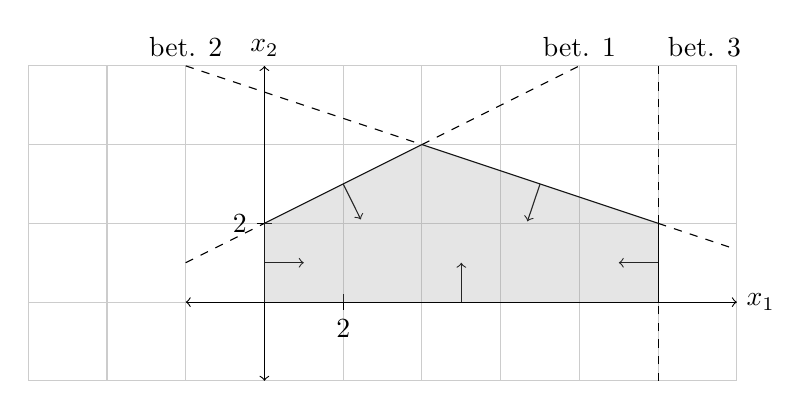
\begin{tikzpicture}
  %laver Grid. godt til når koordinater skal redigeres
  	\draw[thin,gray!40] (-3,-1) grid (6,3); 
  %x-aksen
  	\draw[<->] (-1,0)--(6,0) node[right]{$x_1$};
  	\draw[->] (2.5,0) -- (2.5,0.5);
  %y-aksen
  	\draw[<->] (0,-1)--(0,3) node[above]{$x_2$};
  	\draw[->] (0,0.5) -- (0.5,0.5);
  	
  %akse-markeringer
  	%\node[left] (xakse) at (0,1) {2};
  	\draw[] (-0.1,1) -- (0.1,1) node[pos=0,left] {2};
  	\draw[] (1,-0.1) -- (1,0.1) node[pos=0,below] {2};
  	
  %ligning 1
	\draw[domain=-1:0,variable=\x,dashed] 	plot({\x},{0.5*\x+1});
	\draw[domain=0:2,variable=\x] 			plot({\x},{0.5*\x+1});
	\draw[domain=2:4,variable=\x,dashed] 	plot({\x},{0.5*\x+1}) node[above] {bet. 1};
  	\draw[->] (1,1.5) -- (1.224,1.05);
	
  %ligning 2
  	\draw[domain=-1:2,variable=\x,dashed] 	plot({\x},{-(1/3)*\x+8/3}) node[above] at (-1,3) {bet. 2} ;
	\draw[domain=2:5,variable=\x] 			plot({\x},{-(1/3)*\x+8/3});
	\draw[domain=5:6,variable=\x,dashed] 	plot({\x},{-(1/3)*\x+8/3});
	\draw[->] (3.5,1.5) -- (3.34,1.026);

  %ligning 3
  	\draw[domain=-1:0,variable=\y,dashed] 	plot({5},{\y});
	\draw[domain=0:1,variable=\y] 			plot({5},{\y});
	\draw[domain=1:3,variable=\y,dashed] 	plot({5},{\y}) node[above right] {bet. 3};
	\draw[->] (5,0.5) -- (4.5,0.5);

  %løsningsmængden skraveret
	\fill[gray!80,nearly transparent] (0,0) -- (0,1) -- (2,2) -- (5,1) --(5,0) --  cycle;
\end{tikzpicture}
	\captionof{figure}{Skravering af den mulige mængde for et standard maksimeringsporblem.}
	\label{fig:maksprob2}
\end{center}

\end{eks}

\subsection{Niveaukurver}
En måde at finde den optimale løsning for lineære programmerings problemer med få variable er ved introduktionen af niveaukurver.
\begin{defn}[Niveaukurver]
Lad $f(\vec{x})= \vec{c}^T\vec{x}$ være en funktion, da er en \textbf{niveaukurve} mængden 
\begin{align*}
N_z = \{\vec{x}| f(\vec{x}) = z, z \in \mathds{R}\}
\end{align*}
\end{defn}
Niveau kurver er dermed den mængde af vektorer, der har samme funktionsværdi for objektfunktionen. 
De vektorer udspænder en linje, som er ortogonal med koefficentvektoren $\vec{c}$.
\begin{stn}[Niveaukurven er ortogonal med $\vec{c}$]
Lad $N_z$ betegne en niveaukurve, til objektfunktionen $f(\vec{x})= \vec{c}^T\vec{x}$, da er $\vec{c}$ ortogonal med linjen udspændt af $N_z$.
\end{stn}
\begin{proof}
Lad $\vec{x}, \vec{y} \in N_z$ da er linjen udspændt af $N_z$ parallel med differensvektoren $\vec{x}-\vec{y}$.
Tages prikproduktet af differensvektoren og vektor $\vec{c}$, fåes at
\begin{align*}
\vec{c}^T(\vec{x}-\vec{y}) = \vec{c}^T\vec{x} -\vec{c}^T\vec{y} = z - z = 0,
\end{align*}
hvorfor at vektor $\vec{c}$ og differencevektoren er ortogonale, og dermed må vektor $\vec{c}$ også være orthogonal med linjen udspændt af $N_z$.
\end{proof}
Den optimale løsning findes så ved at finde det mindste $z$ for hvilken niveaukurven har en ikke-tom skæring med den mulige mængde. 
Hvilket gøres ved at flytte kurven så langt i den modsatte retningen af $\vec{c}$ som muligt.
\begin{stn}[Optimal løsning og -værdi fundet ved niveaukurver]
Lad $f(\vec{x})=\vec{c}^T\vec{x}$ betegne objektfunktionen til et standard minimerings problem med løsningsmængde $\mathcal{F}$, da vil den optimale løsning være givet ved 
\begin{align*}
\vec{x^*}=\underset{k}{\min} \, k \cdot \vec{c} \in \mathcal{F}.
\end{align*}
og den optimale værdi er givet ved
\begin{align*}
z^* = \underset{k}{\min} \, k \cdot \Vert \vec{c} \Vert ^2
\end{align*}
\label{stn:niveau}
\end{stn}
\begin{proof}
Det følger af Sætning %mangler
, at en løsningsvektor $\vec{x}$ kan omskrives til summen af en vektor parallel med $\vec{c}$, kaldet $\vec{x}_p$, og en vektor orthogonal med $\vec{c}$, kaldet $\vec{x}_o$. 
Dermed kan objektfunktionen omskrives til
\begin{align*}
	f(\vec{x}) & \ = \ \vec{c}^T\vec{x}\\
	f(\vec{x_p}+\vec{x_o}) & \ = \ 
	\vec{c}^T\vec{x_p}+\vec{c}^T\vec{x_o} \ = \ 
	\vec{c}^T\vec{x_p} \ = \ 
	k\cdot \vec{c}^T\vec{c} \ = \ 
	k \cdot \Vert \vec{c} \Vert ^2.
\end{align*}
Dermed kan det konkluderes at den optimale løsning er en vektor $\vec{x^*}=\underset{k}{min} k \cdot \vec{c} \in \mathcal{F}$, og den optimale værdi er $z* = \underset{k}{min}k \cdot \Vert \vec{c} \Vert ^2$
\end{proof}
Af Sætning \ref{stn:niveau} følger det også, at den optimale værdi er den vinkelrette afstand fra origo og  linjen udspændt af niveaukurven. 
Det følger af at den optimale værdi er givet, som et multiplum af længden af $\vec{c}$, der står vinkelret på linjen udspændt af niveaukurven.
i
Dette kan ses i  for et maksimerings problem i Eksempel \ref{eks:maksprob3}.


\begin{eks}[Optimal løsning fundet grafisk]
Niveaukurverne $46=\vec{c}^T \vec{x}$ og $25=\vec{c}^T \vec{x}$ er på Figur \ref{fig:maksprob3} indtegnet for programmeringsprogblemet fra Eksempel \ref{eks:maksprob2}.

	\begin{center}	
		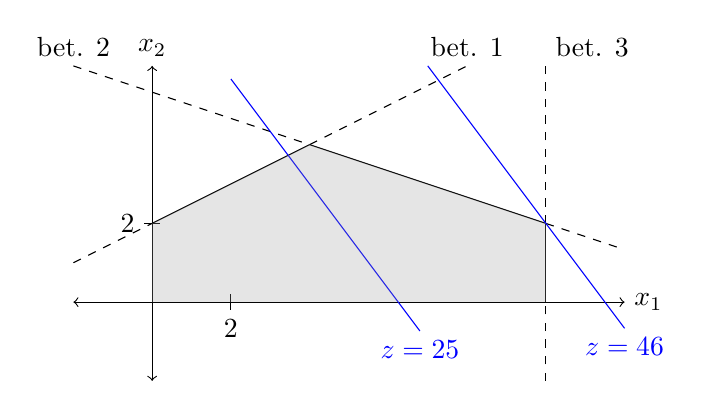
\begin{tikzpicture}
  %laver Grid. godt til når koordinater skal redigeres
  	%\draw[thin,gray!40] (-3,-1) grid (6,3); 
  %x-aksen
  	\draw[<->] (-1,0)--(6,0) node[right]{$x_1$}; 
  %y-aksen
  	\draw[<->] (0,-1)--(0,3) node[above]{$x_2$};
  	
  %akse-markeringer
  	%\node[left] (xakse) at (0,1) {2};
  	\draw[] (-0.1,1) -- (0.1,1) node[pos=0,left] {2};
  	\draw[] (1,-0.1) -- (1,0.1) node[pos=0,below] {2};
  	
  %ligning 1
	\draw[domain=-1:0,variable=\x,dashed] 	plot({\x},{0.5*\x+1});
	\draw[domain=0:2,variable=\x] 			plot({\x},{0.5*\x+1});
	\draw[domain=2:4,variable=\x,dashed] 	plot({\x},{0.5*\x+1}) node[above] {bet. 1};
	
  %ligning 2
  	\draw[domain=-1:2,variable=\x,dashed] 	plot({\x},{-(1/3)*\x+8/3}) node[above] at (-1,3) {bet. 2} ;
	\draw[domain=2:5,variable=\x] 			plot({\x},{-(1/3)*\x+8/3});
	\draw[domain=5:6,variable=\x,dashed] 	plot({\x},{-(1/3)*\x+8/3});
	

  %ligning 3
  	\draw[domain=-1:0,variable=\y,dashed] 	plot({5},{\y});
	\draw[domain=0:1,variable=\y] 			plot({5},{\y});
	\draw[domain=1:3,variable=\y,dashed] 	plot({5},{\y}) node[above right] {bet. 3};
	
  %niveaukurver
  	\draw[domain=3.5:6,variable=\x,blue] plot({\x},{-(4/3)*\x+23/3}) node[below] {$z=46$};
  	\draw[domain=1:3.4,variable=\x,blue] plot({\x},{-(4/3)*\x+25/6}) node[below] {$z=25$};
  	
  %c-vektor
  	%\draw[->,thick,red] (0,0) -- (2,1.5);

  %løsningsmængden skraveret
	\fill[gray!80,nearly transparent] (0,0) -- (0,1) -- (2,2) -- (5,1) --(5,0) --  cycle;
\end{tikzpicture}
		\captionof{figure}{Optimal løsning i den mulige mængde fundet som skæring med ligningen $z=46$.}
		\label{fig:maksprob3}
	\end{center}
	
På figuren ses det, at den største funktionsværdi $z=46$ findes i skæringen mellem bibetingelse 2 og 3.
Ved at løse bibetingelse 2 og 3 som 2 ligninger med 2 ubekendte findes det at den optimale løsning er $\vec{x}=\rvect{10 & 2}^T.$
\label{eks:maksprob3}
\end{eks}



%\chapter{Geometri}
I lineær programmering afsnittet, er løsningerne til et optimeringsproblem beskrevet som værende alle de $\vec{x}$ som overholder bibetingelserne. Dette er beskrevet som værende et polyhedron.
\begin{defn} [Polyhedron]
Et \textbf{Polyhedron} er en mængde 
\begin{align*}
 P =\{ \vec{x} \in \mathds{R}^n | A \vec{x} \geq \vec{b}, \vec{b}\in \mathds{R}^m\},
\end{align*}
hvor at $A$ er en $m \times n$ matrice.
\end{defn}
Hvis et lineært programmerings problem står på standard form $\{ \vec{x} \in \mathds{R}^n | A \vec{x} = \vec{b}, \vec{b}\in \mathds{R}^m\}$, så kaldes dette stadig et polyhedron.\\

Hvis der er en polyhedron $P=\{x|A\vec{x}=\vec{b},x\geq 0\}$ som består af alle bibetingelserne for problemet, så må der også findes en anden polyhedron $Q$, som består af alle de lineære uafhængige bibetingelserne for problemet. Det giver god mening, at fordi $P$ består af de samme bibetingelser som $Q$ og så lidt flere til, så er en løsning $\vec{x}$ til $P$ også en løsning til $Q$ og modsat er en løsning til $Q$ også en løsning til $P$ og derfor må $Q=P$, hvilket vil blive bevist i følgende sætning.

\begin{stn} 
Lad $P=\{\vec{x}|A\vec{x}=\vec{b},x\geq 0\}$ være en ikke-tom polyhedron, hvor $A$ er en $m\times n$ matrix med lineære uafhængige søjler.\\
Antag at $rank(A)=k<m$. Betragt polyhedronen $Q=\{\vec{x}|A_{j_1}\vec{x}=b_{i_1},\dots ,A_{j_k}\vec{x}=b_{i_k}\}$, så er $Q=P$.
\label{stn:PQ}
\end{stn}
\begin{proof}
Hvis $P=\{x|A\vec{x}=\vec{b},x\geq 0\}$ er en polyhedron, der består af alle bibetingelserne og har $rank(A)=k$, så må der være en $Q=\{\vec{x}|A_{j_1}\vec{x}=b_{i_1},\dots ,A_{j_k}\vec{x}=b_{i_k}\}$, der består af alle lineære uafhængig bibetingelser. Så må $P\subset Q$, eftersom alle elementerne i $P$ også tilfredsstiller bibetingelserne for $Q$.\\
Eftersom $rank(A)=k$, så er $k$ rækkerummet af $A$ og så former rækkerne $\vec{a_1},\dots ,\vec{a_k}$ en basis for rækkerummet, derfor kan lineare kombinationen af rækkerne $a_i$ af $A$, skrives som $a_i=\sum_{j=1}^{k}{i j}\vec{a_j}$ for en skalar $c_{i j}$, lad så $\vec{x}$ være en del af $P$ så
\begin{align*}
\vec{a_i}\vec{x}=\sum_{j=1}^{k}c_{i j}\vec{a_j}\vec{x}=\sum_{j=1}^{k}c_{i j}\vec{b_j}=\vec{b_i} \qquad i=1,\dots,m.
\end{align*}
Lad nu $\vec{y}$ være en del af Q, så er $\vec{y}$ også en del af P, eftersom:
\begin{align*}
\vec{a_i}\vec{y}=\sum_{j=1}^{k}c_{i j}\vec{a_j}\vec{y}=\sum_{j=1}^{k}c_{i j}\vec{b_j}=\vec{b_i} \qquad i=1,\dots,m.
\end{align*}
Hvilket betyder $\vec{y}\in P$ og $Q\subset P$ og derved $P=Q$.
\end{proof}

\section{Basisløsninger}

%Jeg har endnu ikke fået gennemgået beviserne til de to sætninger ordentligt. de er bare stjålet fra jer andre.

Basisløsninger danner grundlaget for udregningen af den optimale løsning, hvilket beskrives og anvendes i Kapitel \ref{afsnit:simplex}. For at kunne beskrive netop basisløsninger er det nødvendigt først at introducere definitionen for \textbf{aktive betingelser}.%Ved ikke: Skal vi også bruge fed når ord introduceres i bindende tekst?

\begin{defn}[Aktive betingelser]
En betingelse siges at være \textbf{aktiv} for en givet løsningsvektor $\vec{x}$, hvis det gælder, at\\ $\vec{a}_i^T \vec{x}^* = b_i$.
\label{def:aktiv}
\end{defn}

Generelt bliver aktive betingelser brugt, da de for uligheder repræsenterer en grænse for de mulige løsninger i en given retning, mens de for ligheder blot beskriver, at betingelsen er opfyldt.
Yderligere anvendes skæringen mellem disse aktive betingelser, da den optimale løsning for lineære programmeringsproblemer findes i netop disse skæringer. Hvorfor dette netop er tilfældet bliver begrundet i Afsnit \ref{sec:eksistens}.

\begin{stn}[Lineært uafhængige rækker]
Lad $\vec{x}^* \in \mathds{R}^n$ og $I = \{i | \vec{a_i}^T \vec{x}^* = b_i\}$ være mængden af indekser for aktive betingelser. Da er følgende ækvivalent
\begin{enumerate}[label=(\alph*)]
\item Mængden $R_a =\{\vec{a_i}| i\in I\}$ indeholder vektorer, hvoraf $n$ af dem er lineært uafhængige.
\item Spannet $span(R_a) = \mathds{R}^n$.
\item Ligningssystemet $\vec{a_i}^T \vec{x}^* = b_i$, for $i \in I$ har en unik løsning.
\end{enumerate}
\label{stn:uniklosning}
\end{stn} %Ved ikke: Bør det siges at $\vec{a_i}$ repræcentere en række, eller er det underforstået i rapporten da den altid gør det?

\begin{proof}
	(a) <=> (b): Antag at der i $R_a$ er $n$ lineært uafhængige vektorer. Da der er $n$ lineært uafhængige vektorer må dimensionen af spannet af $R_a$ være $n$. Da $dim(span(R_a))=dim(\mathds{R}^n)=n$ og da $R_a \subseteq \mathds{R}^n$ må det følge af Sætning \ref{stn:dimunderrum} at $span(R_a)=\mathds{R}^n$. Tilsvarende gælder det at hvis $span(R_a)=\mathds{R}^n$, må det gælde at $dim(span(R_a))=dim(\mathds{R}^n)=n$. Da vil kardinaliteten af en basis for $R_a$ nødvendigvis være $n$, hvorved $R_a$ skal indeholde $n$ lineært uafhængige vektorer.


(a) <=> (c): Antag at $span(R_a)=\mathds{R}^n$. Antag nu for modstrid at der findes to løsninger, $\vec{x}_a$ og $\vec{x}_b$ som opfylder $\vec{a}_i\vec{x}=\vec{b}$ for alle $i \in I$. 
Da vil det for alle $i \in I$ gælde at $\vec{a}_i^T\vec{x}_a=\vec{b}$ og at $\vec{a}_i^T\vec{x}_b=\vec{b}$, hvorved $\vec{a}_i^T\vec{d}=\vec{0}$, hvor $\vec{d}=\vec{x}_a-\vec{x}_b$. 
Vektoren $\vec{d}$ vil da være orthogonal på alle $\vec{a}_i$ for $i \in I$ og kan derfor ikke være en lineær kombination af disse. Herved kan $R_a$ ikke udspænde hele $\mathds{R}^n$, da $\vec{d} \in \mathds{R}^n$ men $\vec{d} \notin span(R_a)$.
Tilsvarende antages det nu at der kun er en unik løsning til ligningssystemet. For modstrid antages det at $R_a$ ikke udspænder hele $\mathds{R}^n$ Der kan derved vælges en vektor $\vec{d}$ som er orthogonal til $span(R_a)$ hvorved $\vec{a}_i^T(\vec{x}+\vec{d})=\vec{b}$. derved er $\vec{x}$ ikke en unik løsning og der er opstået modstrid.
\end{proof}
	
	
	
	%Da er disse vektorer en basis for det underrum af $\mathds{R}^n$, som de udspænder. Da $dim(\mathds{R}^n)=dim(R_a)=n$ medfører det af sætning [4.59] at $span(R_a)=\mathds{R}^n$. Tilsvarende gælder det at hvis $span(R_a)=\mathds{R}^n$, må det gælde at $dim(span(R_a))=dim(\mathds{R}^n)=n$. Da vil kardinaliteten af en basis for $R_a$ nødvendigvis være $n$, hvorved $R_a$ skal indeholde $n$ lineært uafhængige vektorer.



%\begin{proof}
%(a) => (c): Lad $A$ være en $n \times n$ matrix bestående af rækkerne $\vec{a_i} \in R_a$, og antag at alle $\vec{a_i}$ er lineært uafhængige. 
%Antag nu for modstrid at ligningssystemet $A\vec{x} = \vec{b}$, hvor $\vec{b}$ har indgangende $b_i$ for $i \in I$, har to løsninger. 
%Da vil $A \vec{x} = \vec{b}$ og $A \vec{y} = \vec{b}$ hvorfor $A(\vec{x}-\vec{y}) = \vec{0}$.
%Derfor må søjlerne enten være lineært afhængige, eller $(\vec{x}-\vec{y})= \vec{0}$.
%Da der er $n$ lineært uafhængige rækker i $A$ må $rank(A) = n$, hvorfor alle søjler er lineært uafhængige, da $A$ er en $n \times n$ matrix.
%Det medfører at $\vec{x}-\vec{y} = \vec{0}$, hvorfor det kan konkluderes at løsningen til ligningssystemet er unikt da $ \vec{x}=\vec{y}$, og der derved er bevist modstrid.
%\\(c) => (a): Antag at der er en unik løsning til $A\vec{x} =\vec{b}$. Det medfører at der er en pivotindgang i hver række hvorved: $rank(A) = n$. hvorfor alle rækker må være lineært uafhængige, da $A$ er en $n \times n$ matrice. % s. 78-79 LinAlg
%\\ (a) => (b): Da $R_a$ består af $n$ linært uafhængige $n$-dimentionelle vektorer, må $R_a$ udgøre en base for $\mathds{R}^n$, hvorfor $span(R_a) = \mathds{R}^n$.
%\\ (b) => (a): Antag for modstrid, at vektorene i $R_a$ ikke er lineært uafhængige, da vil der eksistere en vektor $\vec{a}_i \in R_a$ som er en linear kombination af de andre vektorer, der må derfor eksistere en vektor $A\vec{x} = \vec{0}$, hvor $\vec{x} \neq \vec{0}$.
%Da det kun kan lade sig gøre hvis $\vec{x}$ er ortogonal med alle rækker i $A$, kan $\vec{x}$ ikke være en linear kombination af vektorene i $R_a$.
%Hvorfor at $\vec{x} \notin span(R_a)$.
%Derfor kan $span(R_a) \neq \mathds{R}^n$, hvorfor der er opstået modstrid.
%\end{proof}

\begin{defn}[Basisløsning]
Lad $P$ være en polyide dannet af lineære bibetingelser, og lad $\vec{x}^*\in \mathds{R}^n$. Da er $\vec{x}^*$ en \textbf{basisløsning} hvis
\begin{enumerate}[label=(\alph*)]
\item Alle lighedskrav er aktive
\item Der er $n$ lineært uafhængige aktive betingelser
\end{enumerate}
og en \textbf{mulig basisløsning} hvis
\begin{enumerate}[label=(\alph*)]
\setcounter{enumi}{2}
\item $\vec{x}^*$ opfylder alle krav.
\end{enumerate}
\label{def:basislosning}
\end{defn}

Enhver bibetingelse udspænder et rum, for hvilket betingelsen er opfyldt. Skæringen, af de aktive betingelser, danner derved et rum, som er fællesmængden, af betingelsernes udspændte rum. Skæringen, af en mængde af aktive betingelser, svarer derved til den mulige mængde af disse betingelser. Dog gælder det for basisløsninger pr. Definition \ref{def:basislosning}, at der for en basisløsning $\vec{x}$ skal være $n$ lineært uafhængige aktive betingelser, hvorved en basisløsningen er en unik vektor, hvilket er bevist igennem Sætning \ref{stn:uniklosning}. %Ved ikke, er en vektor og et punkt det samme?

\begin{kor}[Endelig mængde af basisløsninger]
Givet en endelig mængde af bibetingelser, vil der kun eksistere en endelig mængde af basisløsninger og derved også kun en endelig mængde mulige basisløsninger.
\end{kor}

\begin{proof}
Betragt et lineært ligningssystem med $m$ uligheder og løsningsvektorer på formen $\vec{x} \in \mathds{R}^n$, hvor m er et endelige tal.
	Betragt da systemet af $n$ aktive uafhængige lineære uligheder udvalgt af de $m$ uligheder. Da vil dette system ifølge Sætning \ref{stn:uniklosning} kun have en løsning, og denne udvælgelse af uligheder giver derved kun en basisløsning. Da der kun er en endelig mængde af muligheder for at udtrække $n$ af $m$ uligheder på, vil der netop også kun være en endelig mængde af basisløsninger. Da mængden af mulige basisløsninger er en delmængde af mængden af basisløsninger, vil der også kun være en endelig mængde af mulige basisløsninger.
\end{proof}

\begin{stn}[Krav til basisløsninger]
Lad $A\vec{x}=b$, $\vec{x}\geq 0$, hvor $A$ er en $m\times n$ matrix med lineært uafhængige rækker. Da er $\vec{x}^*\in \mathds{R}^n$ en basisløsning hvis og kun hvis $A\vec{x}^*=b, \vec{x}^* \geq 0$, og der eksisterer indekser $B(1), ..., B(m)$ således, at
\begin{enumerate}[label=(\alph*)]
\item Kolonerne $A_{B(1)}, ..., A_{B(m)}$ er lineært uafhængige
\item $x_j = 0$ hvis $j \neq B(1),...,B(m)$.
\end{enumerate}
\end{stn}

\begin{proof}
Først vises at (a) og (b) medfører at $\vec{x}$ er en basisløsning.
Lad $I_m$ være mængden af indeks for de lineært uafhængige søjler  $I_m=\{B(1),\dots,B(m)\}$. Per definition er $\vec{b}=\sum_{j=1}^{n} x_j \vec{A}_j$, hvilket må være det samme som $\vec{b}=\sum_{j\in I_m} x_j \vec{A}_j+\sum_{j\notin I_m} x_j \vec{A}_j$, hvor summeringen er opdelt efter om kolonnerne har indeks $i \in I_m$. 
Ifølge sætningens punkt (b) er $x_j=0$ for $j \notin I_m$. Derved bliver summeringen forkortet til $\vec{b}=\sum_{j\in I}x_j \vec{A}_j$. Da vektorerne $\vec{A}_j$ for $j \in I_m$ er lineært uafhængige vil ligningssystemet nødvendigvis have en unik løsning. Da der er $m$ aktive betingelser, vil det pr. Definition \ref{def:basislosning} at $\vec{x}$ er en basisløsning.

% som er summen af alle de lineære uafhængige rækker og deres løsninger lagt sammen med summen af de lineære afhængige rækker og deres løsninger, men $\vec{x_j}$ til de lineære uafhængige løsninger er er i følge sætningen $x_i = 0$ hvis $i \neq B(1),...,B(m)$ så derfor må ligningen blive $b=\sum_{j\in I_m}^{n}x_j \vec{A}_j+0$,
% 
%så derfor må $\vec{x}$ være en basis løsning.

Herefter vises at det at $\vec{x}$ er en basisløsning medfører (a) og (b). Antag at $\vec{x}$ er en basisløsning og lad $x_j$ for indekser $j \in I_k=\{B(1),\dots B(k)\}$ være alle ikke-nul komponenter af $\vec{x}$.
Eftersom $\vec{x}$ er en basisløsning, så må ligningssystemet af aktive betingelser $\sum_{j=1}^{n}\vec{A}_jx_j=\vec{b}$, hvor $x_j=0$ for $j\notin I_k$ have en unik løsning. Dette gælder da en basisløsning har $n$ uafhængige aktive betingelser, hvilket ifølge Sætning \ref{stn:uniklosning} medfører at systemet har en unik løsning. 
Ligeledes må ligningen $\sum_{j \in I_k}\vec{A}_jx_j=\vec{b}$ have en unik løsning og derfor må kolonerne $\vec{A}_{B(1)}, ..., \vec{A}_{B(k)}$ være lineært uafhængige. Derfor må det gælde at $k \leq m$. % Hvis ikke dette var tilfældet ville der eksistere flere $\vec{x}$ som opfylder ligningssystemet, hvilket modstrider at der er en unik løsning.\\
%Eftersom kolonerne $\vec{A}_{B(1)}, ..., \vec{A}_{B(k)}$ er lineært uafhængige, så må det gælde at $k\leq m$. 
Da $A$ har $m$ lineært uafhængige rækker, må $A$ også have $m$ lineært uafhængige kolonner, hvorved $Col(A)=\mathds{R}^m$.

Den næste del af beviset viser, at der for enhver udvælgelse af indekser $I_k$ findes indekser $I_m$ således at $I_k \subseteq I_m$. 
%Den næste del af beviset viser, at der for enhver udvælgelse af $k$ lineært uafhængige kolonner med indekser $I_k$, gælder at der findes en mængde af $m$ lineært uafhængige kolonner med indekser $I_m$, hvorom det gælder at $I_k \subseteq I_m$.
Altså findes der indekser $B(k+1),...,B(m)$, således at kolonnerne med indekser $B(1),...,B(k),...,B(m)$ er lineært uafhængige. 

Hvis alle $\vec{A}_j$ for $j \notin I_k$ er lineært afhængige af $\vec{A}_j$ for $j \in I_k$, gælder det at $span\left( \vec{A}_{B(1)},...,\vec{A}_{B(k)} \right)=Col(A)=\mathds{R}^m$, hvorved $k=m$. 
Hvis der i stedet eksisterer en kolonne med indeks $j \notin I_k$ som er lineært uafhængig af disse kolonner, kan denne tilføjes til mængden af nu $k+1$ uafhængige vektorer. Denne proces kan gentages $m-k$ gange. Da $i \notin I_m$ medfører at $i \notin I_k$ gælder det derved at $\vec{x}_i =0$ for $i \notin I_m$
\end{proof}

\begin{pro}[Procedure for konstruktion af basisløsninger]
\noindent 1. Vælg $m$ lineært uafhængige koloner $\vec{A}_{B(1)},\dots,\vec{A}_{B(m)}$\\
2. Lad $x_i=0 \,\forall i\neq B(1),\dots,B(m)$\\
3. Løs $A\vec{x}=\vec{b}$ for de ubekendte $x_{B(1)},\dots x_{B(m)}$
\end{pro}

\begin{comment}
Der mangler bare generelt bindetekst mellem sætninger, fra at korollar 6.12 skal introduceres til at kapitlet skal afsluttes og føres videre til naboløsninger
\end{comment}

\subsection{Naboløsninger}

Til den senere anvendelse af simpLeX metoden anvendes også \textbf{naboløsninger}, som er defineret i Definition \ref{def:nabo}. Undersøgelsen af naboløsninger i simpLeX metoden som en metode til at reducere antallet af basisløsninger som skal undersøges når den optimale løsning findes. %Bør omformuleres, er kringlet. Ved ikke: Er det realt det der sker? Ved ikke: Skal SimpLeX staves med stort? Jeg tror da det er det der sker. og simplex er med lille. hermed rettet.

\begin{defn}[Naboløsninger]
	To basisløsninger i $\mathds{R}^n$ siges af være \textbf{naboløsninger}, hvis de deler præcis $n-1$ aktive lineært uafhængige bibetingelser.
	\label{def:nabo}
\end{defn}

Et eksempel på naboløsninger ses i Eksempel \ref{eks:nabo}.

\begin{eks}[Naboløsninger]
De to basisløsninger $\vec{p}=\rvect{4 & 4}^T$ og $\vec{q}=\rvect{10 & 2}^T$ set på Figur \ref{fig:nabo} er naboløsninger, da de har $n-1$ fælles aktive betingelser, hvilket for dette eksempel er 1 betingelse, nemlig betingelse (2). Basisløsningen $\vec{p}$ har (1) og (2) som aktive betingelser, mens $\vec{q}$ har (2) og (3) som aktive betingelser. %ved ikke, om nemlig bør slettes.
	
	\begin{center}
	\begin{tabular}{l	>{$}r<{$}	>{$}r<{$}	>{$}l<{$} r}
	Maksimer 		& 		4x_1	&	+3 x_2	& \\
	med hensyn til 	&  \ \ 	-2 x_1	& 	+4 x_2	& \leq 8 	& \quad (1)\\
					&  		x_1		& 	+3 x_2	& \leq 16	& \quad (2)\\
					&  \ \ 	x_1		& 			& \leq 10	& \quad (3)\\
	og $x_1 \geq 0$ (4), $x_2\geq 0$ (5).
	\end{tabular}
	\end{center}
	
	\begin{center}
	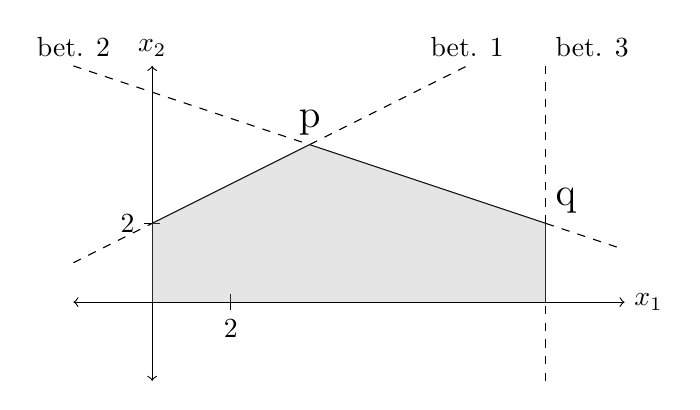
\begin{tikzpicture}
  %laver Grid. godt til når koordinater skal redigeres
  	%\draw[thin,gray!40] (-3,-1) grid (6,3); 
  %x-aksen
  	\draw[<->] (-1,0)--(6,0) node[right]{$x_1$};
  	%\draw[->,red] (2.5,0) -- (2.5,0.5);
  %y-aksen
  	\draw[<->] (0,-1)--(0,3) node[above]{$x_2$};
  	%\draw[->,red] (0,0.5) -- (0.5,0.5);
  	
  %akse-markeringer
  	%\node[left] (xakse) at (0,1) {2};
  	\draw[] (-0.1,1) -- (0.1,1) node[pos=0,left] {2};
  	\draw[] (1,-0.1) -- (1,0.1) node[pos=0,below] {2};
  	
  %ligning 1
	\draw[domain=-1:0,variable=\x,dashed] 	plot({\x},{0.5*\x+1});
	\draw[domain=0:2,variable=\x] 			plot({\x},{0.5*\x+1});
	\draw[domain=2:4,variable=\x,dashed] 	plot({\x},{0.5*\x+1}) node[above] {bet. 1};
  	%\draw[->,red] (1,1.5) -- (1.224,1.05);
	
  %ligning 2
  	\draw[domain=-1:2,variable=\x,dashed] 	plot({\x},{-(1/3)*\x+8/3}) node[above] at (-1,3) {bet. 2} ;
	\draw[domain=2:5,variable=\x] 			plot({\x},{-(1/3)*\x+8/3});
	\draw[domain=5:6,variable=\x,dashed] 	plot({\x},{-(1/3)*\x+8/3});
	%\draw[->,red] (3.5,1.5) -- (3.34,1.026);

  %ligning 3
  	\draw[domain=-1:0,variable=\y,dashed] 	plot({5},{\y});
	\draw[domain=0:1,variable=\y] 			plot({5},{\y});
	\draw[domain=1:3,variable=\y,dashed] 	plot({5},{\y}) node[above right] {bet. 3};
	%\draw[->,red] (5,0.5) -- (4.5,0.5);

  %nodes med navne på punkter
	\node[above] (p) at (2,2) {\Large p};
	\node[above right] (q) at (5,1) {\Large q};

  %løsningsmængden skraveret
	\fill[gray!80,nearly transparent] (0,0) -- (0,1) -- (2,2) -- (5,1) --(5,0) --  cycle;
\end{tikzpicture}
	\captionof{figure}{Løsningsmængde med naboløsninger $p$ og $q$.}
	\label{fig:nabo}
	\end{center}
	
\label{eks:nabo}
\end{eks}

%ved ikke: Må et afsnit slutte med et eksempel?

\section{Optimale løsning}
\label{sec:eksistens}
Hvis løsnings mængden til et lineært programmerings problem ikke er tom, må der være en løsning til problemet.
Men bare fordi der eksistere en løsning, behøver der ikke eksistere en optimal løsning. 
%\begin{defn}
%Lad $P=\{\vec{x} \in \mathds{R}^n| A \vec{x} \geq b, \vec{x} \geq \vec{0}\} \neq \emptyset$ være en polyide, svarende til bibetingelserne til det lineære minimerings problem $\vec{c}^T\vec{x}$.
%Da siges en vektor $\vec{x^*}\in P$ at være \textbf{optimal}, hvis $\vec{c}^T\vec{x^*}\leq \vec{c}^T\vec{x}$ for alle $\vec{x}\in P$
%\end{defn}
Betragt tilfældet, hvor der eksistere en vektor i løsningsmængden, hvor det er muligt at lægge en vilkårlig stor vektor til, og summen stadig er indholdt i løsnings mængden.
Er det tilfældet siges løsningsmængden at indeholde en linje.
\begin{defn}[Linje]
Lad $P\subseteq \mathds{R}^n $ være en polyide, da indeholder $P$ en \textbf{linje}, hvis $\vec{x}+\lambda\vec{d} \in P$ for alle $\lambda \in \mathds{R}^n$, hvor $\vec{x}\in P$ og $\vec{d} \in \mathds{R}^n$.
\end{defn}
Hvis løsningsmængden indholder en linje, så må objektfunktion nødvendigvis kunne tage en vilkårlig stor værdi, og løsningen vil være lig $-\infty$ i tilfældet af, at objektfunktionen skal minimeres. 
Det antyder derfor, at objektfunktionen skal være begrænset, for at der eksistere en optimal løsning.
%\begin{defn} [Begrænset]
%Lad $S \subset \mathds{R}^n$, da er $S$ begrænset, hvis der eksistere en konstant $K$ så $\forall \vec{x} \in S: \langle \vec{x}, \vec{x} \rangle \leq K$
%\end{defn}
Det viser sig, at hvis løsnings mængden ikke er tom og ikke indeholder en linje, så er der en optimal løsning, som vil være en mulig basisløsning, det vil sige, at løsningen findes i et skærings punkt af $n$ lineært uafhængige bibetingelser.
\begin{stn}[Eksistens af optimal løsning]
Lad $P=\{\vec{x} \in \mathds{R}^n| A \vec{x} \geq b \} \neq \emptyset$ være en polyide, svarende til bibetingelserne til det lineære minimerings problem $\vec{c}^T\vec{x}$. Hvis $P$ ikke indeholder en linje, da vil der eksistere en optimal løsning $\vec{x^{**}}$ som er en mulig basisløsning.
\label{stn:eksistens}
\end{stn}
Sætningen bevises med et medføre bevis, ved at finde en vektor $\vec{x}$ i løsningsmængden også konstruere en mulig basisløsning ud fra vektoren. 
Ved at finde en retnings vektor $\vec{d}$, som minimere objektfunktionen, og så lægge et multiplum af $\vec{d}$ til $\vec{x}$ indtil, at summen gør en ny bibetingelse aktiv. 
Det vil altid være muligt at finde sådan en bibetingelse, da løsningsmængden ikke indeholder en linje.
Processen gentages til, vektoren har $n$ lineært uafhængige aktive bibetingelser, se Figur \ref{fig:eksistens}.
\begin{figure}
\begin{center}
	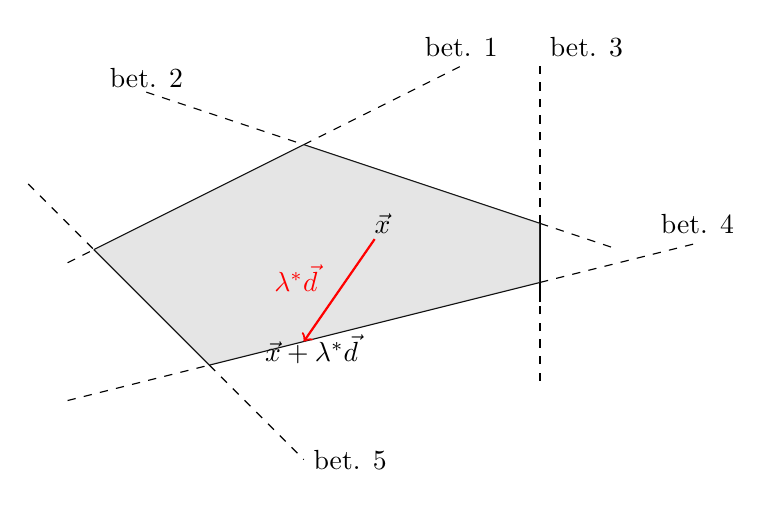
\begin{tikzpicture}[ latex
  s/.style={width=0}]

  %ligning 1
	\draw[domain=-1:-2/3,variable=\x,dashed] 	plot({\x},{0.5*\x+1});
	\draw[domain=-2/3:2,variable=\x] 			plot({\x},{0.5*\x+1});
	\draw[domain=2:4,variable=\x,dashed] 	plot({\x},{0.5*\x+1}) node[above] {bet. 1};
	
  %ligning 2
  	\draw[domain=0:2,variable=\x,dashed] 	plot({\x},{-(1/3)*\x+8/3}) node[above] at (0,2.6) {bet. 2} ;
	\draw[domain=2:5,variable=\x] 			plot({\x},{-(1/3)*\x+8/3});
	\draw[domain=5:6,variable=\x,dashed] 	plot({\x},{-(1/3)*\x+8/3});
	

  %ligning 3
  	\draw[domain=-1:0,variable=\y,dashed] 	plot({5},{\y});
	\draw[domain=0:1,variable=\y] 			plot({5},{\y});
	\draw[domain=1:3,variable=\y,dashed] 	plot({5},{\y}) node[above right] {bet. 3};
	
  %ligning 4
	\draw[domain=-1:4/5,variable=\x,dashed] 	plot({\x},{0.25*\x-1});
	\draw[domain=4/5:5,variable=\x] 			plot({\x},{0.25*\x-1});
	\draw[domain=5:7,variable=\x,dashed] 	plot({\x},{0.25*\x-1}) node[above] {bet. 4};
	
  %ligning 5
  	\draw[domain=-1.5:-2/3,variable=\x,dashed] 	plot({\x},{-\x}) ;
	\draw[domain=-2/3:4/5,variable=\x] 			plot({\x},{-\x});
	\draw[domain=4/5:2,variable=\x,dashed] 	plot({\x},{-\x}) node[right] {bet. 5} ;

  %løsningsmængden skraveret
	\fill[gray!80,nearly transparent] (4/5,-4/5) -- (-2/3,2/3) -- (2,2) -- (5,1) --(5,0.25) --  cycle;
	
  % vektor x
	\node[] (x) at (3,1) {$\vec{x}$};
	\draw[thick, color=red, ->](2.9,0.8) -- (2,-0.5) node[above, yshift=0.5 cm, xshift=-0.1 cm] {$\lambda^* \vec{d}$} ;
	\node[] (x) at (2.1, -0.6) {$\vec{x}+\lambda^* \vec{d}$};
 
\end{tikzpicture}
	\captionof{figure}{Der ligges et multiplum af en retnings vektor til vektor $\vec{x}$ til at summen gør betingelse $4$ aktiv.}
	\label{fig:eksistens}
\end{center}
\end{figure}
Da objektfunktionen til enhver vektor i løsningsmængden, derfor er mindre eller lig objektfunktionen til en mulig basisløsning, må den optimale løsning, være en mulig basisløsning.
\begin{proof}
Da $P$ ikke er tom må der eksistere en vektor $\vec{x} \in P$.
Antag at $\vec{x}$ ikke er en mulig basisløsning, da vil $I = \{i | \vec{a_i}^T\vec{x} = b_i\}$, hvor $\vec{a_i}^T\vec{x}=b_i$ er aktive lineære uafhængige bibetingelser, indeholde færre end $n$ elementer. 
Nu konstrueres en mulig basisløsning $\vec{x^*}$, med udgangspunkt i $\vec{x}$ så $\vec{c}^T\vec{x^*}\leq \vec{c}^T\vec{x}$.
Da $|I|<n $ må $span(\{a_i | i \in I\})$ være et ægte underrum til $\mathds{R}^n$, hvorfor der eksistere en vektor $\vec{d} \in \mathds{R}^n$ så $\vec{a_I}^T\vec{d}=0$ for alle $i \in I$. 
Vælg nu fortegn på $\vec{d}$ så $\vec{c}^T\vec{d} \leq 0$, da vil $\vec{c}^T(\vec{x}+\lambda\vec{d}) \leq \vec{c}^T\vec{x}$ hvor $\lambda$ er en positiv skalar.
Da $P$ er begrænset, og derfor ikke indeholder en linje, må der være et $\lambda'$ som gør, at $\vec{x}+\lambda'\vec{d} \notin P$, hvorfor at der for et $\lambda^*$ må gælde, at $\vec{a_j}^T(\vec{x}+\lambda^* \vec{d}) = b_j$, for $j \notin I$.
Bemærk at $\vec{x}+\lambda^*\vec{d} \in P$, da $\vec{a_i}^T(\vec{x}+\lambda\vec{d})= \vec{a_i}^T\vec{x} = b_i$, for $i \in I$, hvorfor alle aktive bibetingelser stadig er overholdt.
Antag nu at $\vec{d}$ er lineært afhængig af andre bibetingelser end $\vec{a_j}$, da vil $\vec{a_j}$ også være lineært afhæng af dem, hvorfor det følger af Sætning \ref{stn:PQ}, at man kan se bort fra dem, og $\vec{x}+\lambda \vec{d} \in P$ må derfor stadig gøre sig gældende. 
Da $\vec{d}$ er lineært afhængig af $\vec{a_j}$, må det medfører, at da $\vec{d}$ er lineært uafhængig af $\vec{a_i}$ så må $\vec{a_j}$ også være det. 
Derfor kan $j$ tilføjes til $I$. 
Gentag til at $I$ indeholder $n$ lineært uafhængige vektorer, hvorefter det følger af Definition \ref{def:basislosning} at en basisløsning er konstrueret, og da løsningen er konstrueret ud fra en mulig løsning uden at overtræde nogle betingelser, må det være en mulig basisløsning.\\
Da $\vec{x^*}$ er konstrueret ud fra en vilkårlig vektor $\vec{x}\in P$ medføre det, at en mulig basisløsning altid vil opfylde $\vec{c}^T\vec{x^*} \leq \vec{c}\vec{x}$ for en hver ikke mulig basisløsning. 
Da der kun er en endelig mængde mulige basisløsninger, må der være en vektor $\vec{x^{**}}$, som opfylder, at $\vec{c}^T\vec{x^{**}}\leq \vec{c}^T\vec{x^*}$ for alle andre mulige basisløsninger, hvorfor at $\vec{x^{**}}$ er en optimal løsning.
\end{proof}
Sætning \ref{stn:eksistens} kan omskrives en smugle, så i stedet for at kravet er, at løsningsmængden ikke har en linje, så er det at objekt funktionen til løsningsmængden er begrænset.
\begin{kor}
Lad $f(\vec{x}) = \vec{c}^T\vec{x}$ betegne et lineært minimerings programmerings problem, med mulige løsningsmængde $\mathcal{F} \neq \emptyset$. 
Da eksistere en optimal løsning, som er en mulig basisløsning, hvis der eksistere et $K \in \mathds{R}$ så $|f(\mathcal{F})| \leq K$ 
\label{kor:eksistens}
\end{kor}
\begin{proof}
Lad  $K \in \mathds{R}$ så $|f(\mathcal{F})| \leq K$, da må der for et hvert $\vec{x} \in P$ og $\vec{d} \in \mathds{R}^n$ eksistere et $\lambda$ så $f(\vec{x}+\lambda \vec{d}) = K$, og da $f$ er lineær, følger det, at $\mathcal{F}$ ikke kan indeholde en linje. 
Da $\mathcal{F} \neq \emptyset$ følger det af Sætning \ref{stn:eksistens}, at er eksistere en optimal løsning, som er en mulig basisløsning til det lineære minimerings programmerings problem.
\end{proof}
Det betyder, at hvis der til et lineært programmerings problem skal eksistere en optimal løsning, så må løsningsmængden ikke indeholde en linje og objektfunktion på løsningsmængden skal være begrænset. 
Er det ikke tilfældet må objektfunktionen kunne tage værdierne $\infty$ og $-\infty$, og det vil derfor være løsningen på problemet, alt afhængig af om, der er tale om et henholdsvis maksimering eller minimerings problem.





%\endgroup
\chapter{Geometri}
Intro til Geometri
\section{Hvilke typer af mængder beskæftiger vi os med?}
I lineær programmering afsnittet, er løsningerne til et optimeringsproblem beskrevet som værende alle de $\vec{x}$ som overholder bibetingelserne. Dette er beskrevet som værende et polyhedron
\begin{defn} [Polyhedron]
Et \textbf{Polyhedron} er en mængde 
\begin{align*}
 P =\{ \vec{x} \in \mathds{R}^n | A \vec{x} \geq \vec{b}, \vec{b}\in \mathds{R}^m\},
\end{align*}
hvor at $A$ er en $m \times n$ matrice.
\end{defn}
Hvis et lineært programmerings problem står på standard form $\{ \vec{x} \in \mathds{R}^n | A \vec{x} = \vec{b}, \vec{b}\in \mathds{R}^m\}$, så kaldes dette stadig et polyhedron.\\
Et polyhedron kan, alt efter bibetingelserne, være en mængde der strækker sig ud i det uendelige eller de kan være begrænset 
Hvis der er med et maksimerings problem at gøre, kan det ses at bibetingelserne danner et område, men ved at minimeringsproblem, vil bibetingelserne ofte resultere i, at polyheronet strækker ud i det uendelige og derfor ikke længere er en form, men selvom dette er tilfældet, kaldes løsningsmængden stadig for et polyhedron.
følgene definition omhandler et begrænset område
\begin{defn} [Begrænset]
Lad $S \subset \mathds{R}^n$, da er $S$ begrænset, hvis der eksistere en konstant $K$ så $\forall \vec{x} \in S: |\vec{x}| \leq K$
\end{defn}
Med andre ord, hvis der findes en konstant, som er højere end den absolutte værdi af alle $\vec{x} \in S \in S$, hvis der ikke eksistere en konstant, som er støre end $|\vec{x}|$, så ville alle $\vec{x}$ gå mod uendeligt

\begin{defn}
Lad $ \vec{a} \in \mathds{R}^n$, $\vec{a}\neq \vec{0}$ og $b$ være en skalar, da kaldes en mængde for:
\begin{enumerate}
\item En \textbf{Hyperplan} hvis $\{ \vec{x} \in \mathds{R}^n | \vec{a}^{T}\vec{x} = \vec{b}\}$.
\\ \item En \textbf{Halfspace} hvis $\{ \vec{x} \in \mathds{R}^n | \vec{a}^{T} \vec{x} \geq \vec{b}\}$
\end{enumerate}
\end{defn}

\subsection{Konveks}

\begin{defn} [Konveks]
Lad $S \subset \mathds{R}^n$  da er $S$ konveks, hvis der $\forall \vec{x}, \vec{y} \in S$ og et vilkårligt $\lambda \in [0,1]$ gælder at $\lambda \vec{x} + (1-\lambda) \vec{y} \in S$.
\label{def:Konveks}
\end{defn}
Med andre ord så vil ligningen $\lambda \vec{x} + (1-\lambda) \vec{y}$, hvor $\lambda$ ligger i intervallet fra $0$ til $1$, danne en linje af elementer mellem $\vec{x}$ og $\vec{y}$, hvis alle disse elementer er inden som området $S$, så er mængden konveks

\begin{defn}[Konveks kombination og konveks huld]
Lad $\vec{x}^1, ...,\vec{x}^k \in \mathds{R}^n$, og $\lambda_1,..., \lambda_k \geq 0 $ være skalare, som opfylder $\sum_{i=1}^k \lambda_i =1$ da er
\begin{enumerate}[label=(\alph*)]
\item $\sum_{i=1}^k \lambda_i \vec{x}^1$ en \textbf{konveks kombination}.
\\ \item $C_{x} = \{\sum_{i=1}^k \lambda_i \vec{x}^1| \vec{x}^1, ...,\vec{x}^k \in \mathds{R}^n, \sum_{i=1}^k \lambda_i =1\}$ et \textbf{konveks huld} for vektorene $\vec{x}^1, ...,\vec{x}^k$. 
\end{enumerate}
\label{def:KonveksKombination}
\end{defn}

\begin{stn}[Konveks kombination]
Lad $S\subset \mathds{R}^n$ være en konveks mængde, da
\begin{align*}
	\sum_{i=1}^k \lambda_i \vec{x}^i \in S, \qquad \vec{x}^1, ...,\vec{x}^k \in S.
\end{align*}
\label{stn:KonveksKombination}
\end{stn}

\begin{proof}
For at vise Sætning \ref{stn:KonveksKombination} gøres brug af et induktionsbevis.
Lav derfor induktionsstarten ved at betragte den konvekse kombination $\sum_{i=1}^2 \lambda_i \vec{x}^1$.
Da $\sum_{i=1}^2 \lambda_i = \lambda_1 + \lambda_2 = 1$ ifølge Definition \ref{def:KonveksKombination} (a), må $\lambda_2 = (1 - \lambda_1)$.
Det indsættes nu i den konvekse kombination af $\vec{x}^1$ og $\vec{x}^2$, hvorfor at $\lambda_1 \vec{x}^1+ (1-\lambda_1) \vec{x}^2$.
Da $S$ er konveks følger det af Definition \ref{def:Konveks} at $\sum_{i=1}^2 \lambda_i \vec{x}^1 \in S$.
\\Antag derefter at $\sum_{i=1}^k \lambda_i \vec{x}^i \in S$ som induktionshypotesen.
\\ Det vises nu at induktionshypotesen medfører at Sætning \ref{stn:KonveksKombination} også gælder for $k+1$.
Lav derfor induktionstrinnet ved at betragte 
\begin{align*}
	\sum_{i=1}^{k+1} \lambda_i \vec{x}^i &= \lambda_{k+1}\vec{x}^{k+1} + \sum_{i=1}^k \lambda_i \vec{x}^i
	\\ &= \lambda_{k+1}\vec{x}^{k+1} + \frac{1-\lambda_{k+1}}{1-\lambda_{k+1}} \sum_{i=1}^k \lambda_i \vec{x}^i
	\\ &= \lambda_{k+1}\vec{x}^{k+1} + (1-\lambda_{k+1}) \sum_{i=1}^k \frac{1}{1-\lambda_{k+1}} \lambda_i \vec{x}^i
\end{align*}
Observer da at da $\sum_{i=1}^{k+1} \lambda_i \vec{x}^i $ gælder
\begin{align*}
	\sum_{i=1}^{k+1} \lambda_i  & = 1
	\\ \sum_{i=1}^{k} \lambda_i &= 1 - \lambda_{k+1}
	\\ \frac{1}{1-\lambda_{k+1}} \sum_{i=1}^{k} \lambda_i &= \frac{1-\lambda_{k+1}}{1-\lambda_{k+1}} = 1.
\end{align*}
Derfor er $\sum_{i=1}^k \frac{1}{1-\lambda_{k+1}} \lambda_i \vec{x}^i$ en konveks kombination af $k$ elementer, hvorfor det følger af induktionshypotesen at $\sum_{i=1}^k \frac{1}{1-\lambda_{k+1}} \lambda_i \vec{x}^i \in S$, hvorfor at $\sum_{i=1}^{k+1} \lambda_i \vec{x}^i \in S$, og sætningen er bevist.
\end{proof}


\begin{stn}[Konvekse mængder]
Følgende mængder er konvekse
\begin{enumerate}[label=(\alph*)]
\item $A \cap B$, hvis mængderne $A,B$ er konvekse
\\  \item polyhedronet $P =\{ \vec{x} \in \mathds{R}^n | A \vec{x} \geq \vec{b}\} $
\\ \item Konveks huldet $C_x = \{\sum_{i=1}^k \lambda_i \vec{x}^1| \vec{x}^1, ...,\vec{x}^k \in \mathds{R}^n, \sum_{i=1}^k \lambda_i =1\}$ over en endelig mængde vektorer
\end{enumerate}
\end{stn}

\begin{proof}
Først vises udsagn (a).
Lad $\vec{x}, \vec{y} \in A,B$ være to vilkårlige vektorer, da både $A$ og $B$ er konvekse må $\lambda\vec{x} + (1-\lambda) \vec{y} \in A, B$, hvor $ \lambda \in [0,1]$ er en skalar.
Derfor må $\lambda\vec{x} + (1-\lambda) \vec{y} \in  A \cap B$, hvilket medføre af Definition \ref{def:Konveks} at $A \cap B$ er konveks.
\\Så vis udsagn (b).
Lad $\vec{x}, \vec{y} \in P=\{ \vec{x} \in \mathds{R}^n | A \vec{x} \geq \vec{b}\}$ være to vilkårlige vektorer, da gælder at $A\vec{x} \geq \vec{b}$ hvilket medfører at $\lambda A \vec{x} \geq \lambda\vec{b}$, hvor $\lambda \in [0,1]$ er en skalar. 
På ligefod må der derfor gælde at $(1-\lambda)A\vec{y} \geq (1-\lambda)\vec{b}$.
De to uligheder adderes nu
\begin{align*}
\lambda A \vec{x} + (1-\lambda) A \vec{y} \geq \lambda \vec{b} + (1 - \lambda) \vec{b}
\\  A (\lambda\vec{x} + (1-\lambda)\vec{y}) \geq \vec{b}.
\end{align*}
Derfor må $\lambda\vec{x} + (1-\lambda)\vec{y} \in P$.
\\Tilsidst vises udsagn (c).
Lad $\vec{z}, \vec{y}\in C_x = \{\sum_{i=1}^k \lambda_i \vec{x}^i| \vec{x}^1, ...,\vec{x}^k \in \mathds{R}^n, \sum_{i=1}^k \lambda_i =1\}$ være vilkårlige vektorer da må $\vec{z}= \sum_{i=1}^k \gamma_i \vec{x}^i, \vec{y}= \sum_{i=1}^k \eta_i \vec{x}^i$ for $\sum_{i=1}^k \gamma_i = 1$ og  $\sum_{i=1}^k \eta_i = 1$. 
Derfor må
\begin{align*}
	\lambda \vec{z} + (1- \lambda) \vec{y} &= \lambda\sum_{i=1}^k \gamma_i \vec{x}^i + (1-\lambda)\sum_{i=1}^k \eta_i \vec{x}^i
	\\ &=\sum_{i=1}^k (\lambda \gamma_i+(1-\lambda)\eta_i )\vec{x}^i,
\end{align*}
For $\lambda \in [0,1]$.
Betragt nu konstanterne 
\begin{align*}
	\sum_{i=1}^k (\lambda \gamma_i+(1-\lambda)\eta_i ) &= \lambda \sum_{i=1}^k \gamma_i + (1 - \lambda) \sum_{i=1}^k \eta_i 
	\\ &= \lambda \cdot 1 + (1 - \lambda) \cdot 1 = 1
\end{align*}
Hvorfor at $\lambda \vec{z} + (1- \lambda) \vec{y} $ er en konveks kombination af vektorene $\vec{x}^1, ...,\vec{x}^k $, ifølge Definition \ref{def:KonveksKombination}. 
Derfor må $ \lambda \vec{z} + (1- \lambda) \vec{y} \in C_x$, hvorfor at $C_x$ er konveks ifølge Definition \ref{def:Konveks}.
Og sætningen er bevist.
\end{proof}



\section{Basisløsninger}

%Jeg har endnu ikke fået gennemgået beviserne til de to sætninger ordentligt. de er bare stjålet fra jer andre.

Basisløsninger danner grundlaget for udregningen af den optimale løsning, hvilket beskrives og anvendes i Kapitel \ref{afsnit:simplex}. For at kunne beskrive netop basisløsninger er det nødvendigt først at introducere definitionen for \textbf{aktive betingelser}.%Ved ikke: Skal vi også bruge fed når ord introduceres i bindende tekst?

\begin{defn}[Aktive betingelser]
En betingelse siges at være \textbf{aktiv} for en givet løsningsvektor $\vec{x}^*$, hvis det gælder, at\\ $\vec{a}_i^T \vec{x}^* = b_i$.
\label{def:aktiv}
\end{defn}

Generelt bliver aktive betingelser brugt, da de for uligheder repræsenterer en grænse for de mulige løsninger i en given retning, mens de for ligheder blot beskriver, at betingelsen er opfyldt.
Yderligere anvendes skæringen mellem disse aktive betingelser, da den optimale løsning for lineære programmeringsproblemer findes i netop disse skæringer. Hvorfor dette netop er tilfældet bliver begrundet i Afsnit \ref{sec:eksistens}.

\begin{stn}[Lineært uafhængige rækker]
Lad $\vec{x}^* \in \mathds{R}^n$ og $I = \{i | \vec{a_i}^T \vec{x}^* = b_i\}$ være mængden af indekser for aktive betingelser. Da er følgende udsagn ækvivalente:
\begin{enumerate}[label=(\alph*)]
\item Mængden $R_a =\{\vec{a_i}| i\in I\}$ indeholder vektorer, hvoraf $n$ af dem er lineært uafhængige.
\item Spannet $span(R_a) = \mathds{R}^n$.
\item Ligningssystemet $\vec{a_i}^T \vec{x}^* = b_i$, for $i \in I$ har en unik løsning.
\end{enumerate}
\label{stn:uniklosning}
\end{stn} %Ved ikke: Bør det siges at $\vec{a_i}$ repræcentere en række, eller er det underforstået i rapporten da den altid gør det?

\begin{proof}
	(a) <=> (b): Antag at der i $R_a$ er $n$ lineært uafhængige vektorer. Da der er $n$ lineært uafhængige vektorer må dimensionen af spannet af $R_a$ være $n$. Da $dim(span(R_a))=dim(\mathds{R}^n)=n$ og da $R_a \subseteq \mathds{R}^n$ må det følge af Sætning \ref{stn:dimunderrum} at $span(R_a)=\mathds{R}^n$. Tilsvarende gælder det at hvis $span(R_a)=\mathds{R}^n$, må det gælde at $dim(span(R_a))=dim(\mathds{R}^n)=n$. Da vil kardinaliteten af en basis for $R_a$ nødvendigvis være $n$, hvorved $R_a$ skal indeholde $n$ lineært uafhængige vektorer.


(a) <=> (c): Antag at $span(R_a)=\mathds{R}^n$. Antag nu for modstrid, at der findes to løsninger, $\vec{x}_a$ og $\vec{x}_b$, som opfylder $\vec{a}_i\vec{x}=\vec{b}$ for alle $i \in I$. 
Da vil det for alle $i \in I$ gælde at $\vec{a}_i^T\vec{x}_a=\vec{b}$ og at $\vec{a}_i^T\vec{x}_b=\vec{b}$, hvorved $\vec{a}_i^T\vec{d}=\vec{0}$, hvor $\vec{d}=\vec{x}_a-\vec{x}_b$. 
Vektoren $\vec{d}$ vil da være orthogonal på alle $\vec{a}_i$ for $i \in I$ og kan derfor ikke være en lineær kombination af disse. Herved kan $R_a$ ikke udspænde hele $\mathds{R}^n$, da $\vec{d} \in \mathds{R}^n$ men $\vec{d} \notin span(R_a)$.
Tilsvarende antages det nu at der kun er en unik løsning til ligningssystemet. For modstrid antages det at $R_a$ ikke udspænder hele $\mathds{R}^n$ Der kan derved vælges en vektor $\vec{d}$ som er orthogonal til $span(R_a)$ hvorved $\vec{a}_i^T(\vec{x}+\vec{d})=\vec{b}$. Derved er $\vec{x}$ ikke en unik løsning og der er opstået modstrid.
\end{proof}
	
	
	
	%Da er disse vektorer en basis for det underrum af $\mathds{R}^n$, som de udspænder. Da $dim(\mathds{R}^n)=dim(R_a)=n$ medfører det af sætning [4.59] at $span(R_a)=\mathds{R}^n$. Tilsvarende gælder det at hvis $span(R_a)=\mathds{R}^n$, må det gælde at $dim(span(R_a))=dim(\mathds{R}^n)=n$. Da vil kardinaliteten af en basis for $R_a$ nødvendigvis være $n$, hvorved $R_a$ skal indeholde $n$ lineært uafhængige vektorer.



%\begin{proof}
%(a) => (c): Lad $A$ være en $n \times n$ matrix bestående af rækkerne $\vec{a_i} \in R_a$, og antag at alle $\vec{a_i}$ er lineært uafhængige. 
%Antag nu for modstrid at ligningssystemet $A\vec{x} = \vec{b}$, hvor $\vec{b}$ har indgangende $b_i$ for $i \in I$, har to løsninger. 
%Da vil $A \vec{x} = \vec{b}$ og $A \vec{y} = \vec{b}$ hvorfor $A(\vec{x}-\vec{y}) = \vec{0}$.
%Derfor må søjlerne enten være lineært afhængige, eller $(\vec{x}-\vec{y})= \vec{0}$.
%Da der er $n$ lineært uafhængige rækker i $A$ må $rank(A) = n$, hvorfor alle søjler er lineært uafhængige, da $A$ er en $n \times n$ matrix.
%Det medfører at $\vec{x}-\vec{y} = \vec{0}$, hvorfor det kan konkluderes at løsningen til ligningssystemet er unikt da $ \vec{x}=\vec{y}$, og der derved er bevist modstrid.
%\\(c) => (a): Antag at der er en unik løsning til $A\vec{x} =\vec{b}$. Det medfører at der er en pivotindgang i hver række hvorved: $rank(A) = n$. hvorfor alle rækker må være lineært uafhængige, da $A$ er en $n \times n$ matrice. % s. 78-79 LinAlg
%\\ (a) => (b): Da $R_a$ består af $n$ linært uafhængige $n$-dimentionelle vektorer, må $R_a$ udgøre en base for $\mathds{R}^n$, hvorfor $span(R_a) = \mathds{R}^n$.
%\\ (b) => (a): Antag for modstrid, at vektorene i $R_a$ ikke er lineært uafhængige, da vil der eksistere en vektor $\vec{a}_i \in R_a$ som er en linear kombination af de andre vektorer, der må derfor eksistere en vektor $A\vec{x} = \vec{0}$, hvor $\vec{x} \neq \vec{0}$.
%Da det kun kan lade sig gøre hvis $\vec{x}$ er ortogonal med alle rækker i $A$, kan $\vec{x}$ ikke være en linear kombination af vektorene i $R_a$.
%Hvorfor at $\vec{x} \notin span(R_a)$.
%Derfor kan $span(R_a) \neq \mathds{R}^n$, hvorfor der er opstået modstrid.
%\end{proof}

\begin{defn}[Basisløsning]
Lad $P$ være et polyeder dannet af lineære bibetingelser, og lad $\vec{x}^*\in \mathds{R}^n$. Da er $\vec{x}^*$ en \textbf{basisløsning}, hvis
\begin{enumerate}[label=(\alph*)]
\item Alle lighedskrav er aktive
\item Der er $n$ lineært uafhængige aktive betingelser
\end{enumerate}
og en \textbf{mulig basisløsning}, hvis
\begin{enumerate}[label=(\alph*)]
\setcounter{enumi}{2}
\item $\vec{x}^*$ opfylder alle krav.
\end{enumerate}
\label{def:basislosning}
\end{defn}

Enhver bibetingelse udspænder et rum, for hvilket betingelsen er opfyldt. Skæringen, af de aktive betingelser, danner derved et rum, som er fællesmængden af betingelsernes udspændte rum. Skæringen af en mængde af aktive betingelser svarer derved til den mulige mængde af disse betingelser. Dog gælder det for basisløsninger pr. Definition \ref{def:basislosning}, at der for en basisløsning $\vec{x}$ skal være $n$ lineært uafhængige aktive betingelser, hvorved en basisløsningen er en unik vektor, hvilket er bevist igennem Sætning \ref{stn:uniklosning}. %Ved ikke, er en vektor og et punkt det samme?

\begin{kor}[Endelig mængde af basisløsninger]
Givet en endelig mængde af bibetingelser, vil der kun eksistere en endelig mængde af basisløsninger og derved også kun en endelig mængde mulige basisløsninger.
\label{kor:endeligbasis}
\end{kor}

\begin{proof}
Betragt et lineært ligningssystem med $m$ uligheder og løsningsvektorer på formen $\vec{x} \in \mathds{R}^n$, hvor m er et endeligt tal.
	Betragt da systemet af $n$ aktive uafhængige lineære uligheder udvalgt af de $m$ uligheder. Da vil dette system ifølge Sætning \ref{stn:uniklosning} kun have en løsning, og denne udvælgelse af uligheder giver derved kun en basisløsning. Da der kun er en endelig mængde af muligheder for at udtrække $n$ af $m$ uligheder på, vil der netop også kun være en endelig mængde af basisløsninger. Da mængden af mulige basisløsninger er en delmængde af mængden af basisløsninger, vil der også kun være en endelig mængde af mulige basisløsninger.
\end{proof}

\begin{stn}[Krav til basisløsninger]
Lad $A\vec{x}=b$, $\vec{x}\geq 0$, hvor $A$ er en $m\times n$ matrix med lineært uafhængige rækker. Da er $\vec{x}^*\in \mathds{R}^n$ en basisløsning hvis og kun hvis $A\vec{x}^*=b, \vec{x}^* \geq 0$, og der eksisterer indekser $B(1), ..., B(m)$ således, at
\begin{enumerate}[label=(\alph*)]
\item Kolonerne $A_{B(1)}, ..., A_{B(m)}$ er lineært uafhængige og
\item $x_j = 0$, hvis $j \neq B(1),...,B(m)$.
\end{enumerate}
\label{stn:kravtilbasis}
\end{stn}

\begin{proof}
Først vises at (a) og (b) medfører at $\vec{x}$ er en basisløsning.
Lad $I_m$ være mængden af indeks for de lineært uafhængige søjler  $I_m=\{B(1),\dots,B(m)\}$. Per definition er $\vec{b}=\sum_{j=1}^{n} x_j \vec{A}_j$, hvilket må være det samme som $\vec{b}=\sum_{j\in I_m} x_j \vec{A}_j+\sum_{j\notin I_m} x_j \vec{A}_j$, hvor summeringen er opdelt efter om kolonnerne har indeks $i \in I_m$. 
Ifølge sætningens punkt (b) er $x_j=0$ for $j \notin I_m$. Derved bliver summeringen forkortet til $\vec{b}=\sum_{j\in I}x_j \vec{A}_j$. Da vektorerne $\vec{A}_j$ for $j \in I_m$ er lineært uafhængige vil ligningssystemet nødvendigvis have en unik løsning. Da ligningssystemet har en unik løsning gælder det af Sætning \ref{stn:uniklosning}, at ligningssystemet har $n$ lineært uafhængige rækker, som alle er aktive. Da der er $n$ aktive betingelser og da alle lighedskrav er aktive, vil det pr. Definition \ref{def:basislosning} sige at $\vec{x}$ er en basisløsning.

% som er summen af alle de lineære uafhængige rækker og deres løsninger lagt sammen med summen af de lineære afhængige rækker og deres løsninger, men $\vec{x_j}$ til de lineære uafhængige løsninger er er i følge sætningen $x_i = 0$ hvis $i \neq B(1),...,B(m)$ så derfor må ligningen blive $b=\sum_{j\in I_m}^{n}x_j \vec{A}_j+0$,
% 
%så derfor må $\vec{x}$ være en basis løsning.

Herefter vises at det at $\vec{x}$ er en basisløsning medfører (a) og (b). Antag at $\vec{x}$ er en basisløsning og lad $x_j$ for indekser $j \in I_k=\{B(1),\dots B(k)\}$ være alle ikke-nul komponenter af $\vec{x}$.
Eftersom $\vec{x}$ er en basisløsning, så må ligningssystemet af aktive betingelser $\sum_{j=1}^{n}\vec{A}_jx_j=\vec{b}$, hvor $x_j=0$ for $j\notin I_k$ have en unik løsning. Dette gælder da en basisløsning har $n$ lineært uafhængige aktive betingelser, hvilket ifølge Sætning \ref{stn:uniklosning} medfører at systemet har en unik løsning. 
Ligeledes må ligningen $\sum_{j \in I_k}\vec{A}_jx_j=\vec{b}$ have en unik løsning og derfor må kolonerne $\vec{A}_{B(1)}, ..., \vec{A}_{B(k)}$ være lineært uafhængige. Derfor må det gælde at $k \leq m$. % Hvis ikke dette var tilfældet ville der eksistere flere $\vec{x}$ som opfylder ligningssystemet, hvilket modstrider at der er en unik løsning.\\
%Eftersom kolonerne $\vec{A}_{B(1)}, ..., \vec{A}_{B(k)}$ er lineært uafhængige, så må det gælde at $k\leq m$. 
Da $A$ har $m$ lineært uafhængige rækker, må $A$ også have $m$ lineært uafhængige kolonner, hvorved $Col(A)=\mathds{R}^m$.

Den næste del af beviset viser, at der for enhver udvælgelse af indekser $I_k$ findes indekser $I_m$ således at $I_k \subseteq I_m$. 
%Den næste del af beviset viser, at der for enhver udvælgelse af $k$ lineært uafhængige kolonner med indekser $I_k$, gælder at der findes en mængde af $m$ lineært uafhængige kolonner med indekser $I_m$, hvorom det gælder at $I_k \subseteq I_m$.
Altså findes der indekser $B(k+1),...,B(m)$, således at kolonnerne med indekser $B(1),...,B(k),...,B(m)$ er lineært uafhængige. 

Hvis alle $\vec{A}_j$ for $j \notin I_k$ er lineært afhængige af $\vec{A}_j$ for $j \in I_k$, gælder det at $span\left( \vec{A}_{B(1)},...,\vec{A}_{B(k)} \right)=Col(A)=\mathds{R}^m$, hvorved $k=m$. 
Hvis der i stedet eksisterer en kolonne med indeks $j \notin I_k$ som er lineært uafhængig af disse kolonner, kan denne tilføjes til mængden af nu $k+1$ uafhængige vektorer. Denne proces kan gentages $m-k$ gange. Da $i \notin I_m$ medfører at $i \notin I_k$ gælder det derved at $\vec{x}_i =0$ for $i \notin I_m$
\end{proof}

\begin{pro}[Procedure for konstruktion af basisløsninger]
\noindent 1. Vælg $m$ lineært uafhængige koloner $\vec{A}_{B(1)},\dots,\vec{A}_{B(m)}$\\
2. Lad $x_i=0 \,\forall i\neq B(1),\dots,B(m)$\\
3. Løs $A\vec{x}=\vec{b}$ for de ubekendte $x_{B(1)},\dots x_{B(m)}$
\end{pro}

\begin{comment}
Der mangler bare generelt bindetekst mellem sætninger, fra at korollar 6.12 skal introduceres til at kapitlet skal afsluttes og føres videre til naboløsninger
\end{comment}

\subsection{Naboløsninger}

Til den senere anvendelse af simplex metoden anvendes også \textbf{naboløsninger}, som er defineret i Definition \ref{def:nabo}. Undersøgelsen af naboløsninger i simplex metoden som en metode til at reducere antallet af basisløsninger, som skal undersøges når den optimale løsning findes. %Bør omformuleres, er kringlet. Ved ikke: Er det realt det der sker? Ved ikke: Skal SimpLeX staves med stort? Jeg tror da det er det der sker. og simplex er med lille. hermed rettet.

\begin{defn}[Naboløsninger]
	To basisløsninger i $\mathds{R}^n$ siges af være \textbf{naboløsninger}, hvis de deler præcis $n-1$ aktive lineært uafhængige bibetingelser.
	\label{def:nabo}
\end{defn}

Et eksempel på naboløsninger ses i Eksempel \ref{eks:nabo}.

\begin{eks}[Naboløsninger]
De to basisløsninger $\vec{p}=\rvect{4 & 4}^T$ og $\vec{q}=\rvect{10 & 2}^T$ set på Figur \ref{fig:nabo} er naboløsninger, da de har $n-1$ fælles aktive betingelser, hvilket for dette eksempel er $1$ betingelse, nemlig betingelse (2). Basisløsningen $\vec{p}$ har (1) og (2) som aktive betingelser, mens $\vec{q}$ har (2) og (3) som aktive betingelser. %ved ikke, om nemlig bør slettes.
	
	\begin{center}
	\begin{tabular}{l	>{$}r<{$}	>{$}r<{$}	>{$}l<{$} r}
	Maksimer 		& 		4x_1	&	+3 x_2	& \\
	med hensyn til 	&  \ \ 	-2 x_1	& 	+4 x_2	& \leq 8 	& \quad (1)\\
					&  		x_1		& 	+3 x_2	& \leq 16	& \quad (2)\\
					&  \ \ 	x_1		& 			& \leq 10	& \quad (3)\\
	og $x_1 \geq 0$ (4), $x_2\geq 0$ (5).
	\end{tabular}
	\end{center}
	
	\begin{center}
	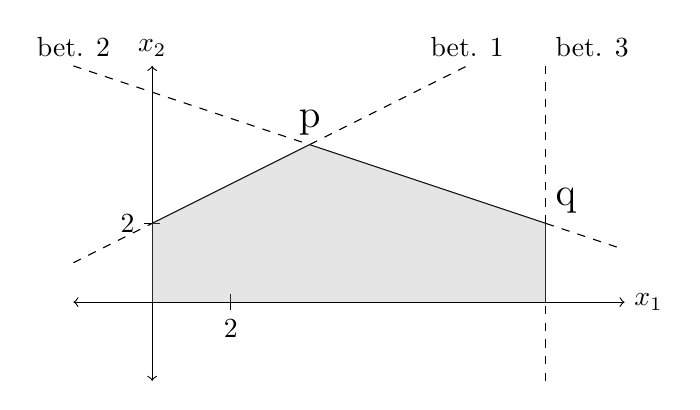
\begin{tikzpicture}
  %laver Grid. godt til når koordinater skal redigeres
  	%\draw[thin,gray!40] (-3,-1) grid (6,3); 
  %x-aksen
  	\draw[<->] (-1,0)--(6,0) node[right]{$x_1$};
  	%\draw[->,red] (2.5,0) -- (2.5,0.5);
  %y-aksen
  	\draw[<->] (0,-1)--(0,3) node[above]{$x_2$};
  	%\draw[->,red] (0,0.5) -- (0.5,0.5);
  	
  %akse-markeringer
  	%\node[left] (xakse) at (0,1) {2};
  	\draw[] (-0.1,1) -- (0.1,1) node[pos=0,left] {2};
  	\draw[] (1,-0.1) -- (1,0.1) node[pos=0,below] {2};
  	
  %ligning 1
	\draw[domain=-1:0,variable=\x,dashed] 	plot({\x},{0.5*\x+1});
	\draw[domain=0:2,variable=\x] 			plot({\x},{0.5*\x+1});
	\draw[domain=2:4,variable=\x,dashed] 	plot({\x},{0.5*\x+1}) node[above] {bet. 1};
  	%\draw[->,red] (1,1.5) -- (1.224,1.05);
	
  %ligning 2
  	\draw[domain=-1:2,variable=\x,dashed] 	plot({\x},{-(1/3)*\x+8/3}) node[above] at (-1,3) {bet. 2} ;
	\draw[domain=2:5,variable=\x] 			plot({\x},{-(1/3)*\x+8/3});
	\draw[domain=5:6,variable=\x,dashed] 	plot({\x},{-(1/3)*\x+8/3});
	%\draw[->,red] (3.5,1.5) -- (3.34,1.026);

  %ligning 3
  	\draw[domain=-1:0,variable=\y,dashed] 	plot({5},{\y});
	\draw[domain=0:1,variable=\y] 			plot({5},{\y});
	\draw[domain=1:3,variable=\y,dashed] 	plot({5},{\y}) node[above right] {bet. 3};
	%\draw[->,red] (5,0.5) -- (4.5,0.5);

  %nodes med navne på punkter
	\node[above] (p) at (2,2) {\Large p};
	\node[above right] (q) at (5,1) {\Large q};

  %løsningsmængden skraveret
	\fill[gray!80,nearly transparent] (0,0) -- (0,1) -- (2,2) -- (5,1) --(5,0) --  cycle;
\end{tikzpicture}
	\captionof{figure}{Løsningsmængde med naboløsninger $p$ og $q$.}
	\label{fig:nabo}
	\end{center}
	
\label{eks:nabo}
\end{eks}

%ved ikke: Må et afsnit slutte med et eksempel?





%\section{Hvad er en løsning?}


\begin{defn}[Ekstremuspunkt]
Lad $\vec{x} \in P$, hvor $P$ er en polyeder og $\lambda \in [0,1]$ være en skalar.
Da er $\vec{x}$ et ekstremuspunkt hvis $\nexists \vec{y}, \vec{z} \in P$ så $\vec{x} = \lambda \vec{y}+ (1- \lambda)\vec{z}$ for $\vec{y}\neq \vec{x}$ og $\vec{z}\neq \vec{x}$.
\end{defn}

\begin{defn}[Knude]
Lad $\vec{x} \in P$, hvor $P$ er en polyeder, da er $\vec{x}$ en knude, hvis $\exists \vec{c} $ så $\vec{c}^T \vec{x} < \vec{c}^T\vec{y}$ $\forall \vec{y} \in P$ for $\vec{y} \neq \vec{x}$.
\end{defn}


\begin{defn}[Aktive krav]
Lad $\vec{x}^* \in \mathds{R}^n$ opfylde at $\vec{a}_i^T\vec{x}^* = b_i$, hvor $\vec{a}_i$ svare til en bibetingelse, da siges $\vec{a_i}^T$ at være \textbf{aktiv}.
\end{defn}

\begin{stn}[Lineær uafhængige rækker]
Lad $\vec{x}^* \in \mathds{R}^n$ og $I = \{i | \vec{a_i}^T \vec{x}^*\geq b_i\}$ , da er følgende ækvivalent
\begin{enumerate}[label=(\alph*)]
\item Mængden $R_a =\{\vec{a_i}| i\in I\}$ består af $n$ elementer, som er lineært uafhængige.
\item Spannet $span(\vec{a_i}) = \mathds{R}^n$, for $a_i \in R_a$.
\item Ligningssystemet $\vec{a_i}^T \vec{x}^* = b_i$, for $a_i \in R_a$ har en unik løsning.
\end{enumerate}
\end{stn}

\begin{proof}
(a) => (c): Lad $A$ være en $n \times n$ matrix bestående af rækkerne $\vec{a_i}^T \in R_a$, og antag at alle $\vec{a_i}$ er lineært uafhængige. 
Antag nu for modstrid at ligningssystemet $A\vec{x} = \vec{b}$, hvor $\vec{b}$ har indgangende $b_i$ for $i \in I$, har to løsninger. 
Da vil $A \vec{x} = \vec{b}$ og $A \vec{y} = \vec{b}$ hvorfor $A\vec{x-y} = \vec{0}$.
Derfor må søjlerne enten være lineært afhængige, eller $\vec{x-y} = \vec{0}$.
Da der er $n$ lineært uafhængige rækker i $A$ må $rank(A) = n$, hvorfor alle søjler er lineært uafhængige, da $A$ er en $n \times n$ matrice.
Det medfører at $\vec{x-y} = \vec{0}$, hvorfor det kan konkluderes at løsningen til ligningssystemet er unikt da $ \vec{x}=\vec{y}$.
\\(c) => (a):Antag at der er en unik løsning til $A$ det medfører at $rank(A) = n$, hvorfor alle rækker må være lineært uafhængige, , da $A$ er en $n \times n$ matrice. % s. 78-79 LinAlg
\\ (a) => (b): Da $R_a$ består af $n$ linært uafhængige $n$-dimentionelle vektorer, må $R_a$ udgøre en base for $\mathds{R}^n$, hvorfor $span(R_a) = \mathds{R}^n$.
\\ (b) => (a): Antag for modstrid, at vektorene i $R_a$ ikke er lineært uafhængige, da vil der eksistere en vektor $\vec{a_i'} \in R_a$ som er en linear kombination af de andre vektorer, der må derfor eksistere en vektor $A\vec{x} = \vec{0}$, hvor $\vec{x} \neq \vec{0}$, da det kun kan lade sig gøre hvis $\vec{x}$ er ortogonal med alle rækker i $A$, kan $\vec{x}$ ikke være en linear kombination af vektorene i $R_a$.
Hvorfor at $\vec{x} \notin span(R_a)$.
Derfor kan $span(R_a) \neq \mathds{R}^n$, hvorfor der er opstået modstrid.
\end{proof}





\begin{defn}[Basis løsning]
$P$, $\vec{x}^*\in \mathds{R}^n$, da er $\vec{x}^*$ en \textbf{Basis løsning} hvis:
\begin{enumerate}[label=(\alph*)]
\item Alle ligheds krav er aktive
\item der er mindst $n$ lineært uafhængige aktive krav
\end{enumerate}
og en \textbf{Mulig basis løsning} hvis:
\begin{itemize}
\item $\vec{x}^*$ opfylder alle krav.
\end{itemize}
\end{defn}


    

\begin{stn}[Løsningerne er de samme]
$\vec{x}^* \in P$ da er følgende ækvivalent:
\begin{enumerate}[label=(\alph*)]
\item ekstremuspunkt
 \item node
 \item mulig basis løsning
\end{enumerate}
\end{stn}


\begin{cor}
Endeligt antal krav medføre endeligt antal basisløsninger
\end{cor}

\begin{defn}[Naboløsninger]
Naboløsninger, har samme aktive krav pånær et
\end{defn}

\begin{stn}[Er en basisløsning når:]
Krav $A\vec{x}=b$, $\vec{x}\geq 0$, hvor $A$ er $m\times n$ matrix med lineært uafhænginge rækker. Da er $\vec{x}^*\in \mathds{R}^n$  basis løsning hviss $A\vec{x}^*=b, \vec{x}^* \geq 0$, og der $\exists B(1), ..., B(m)$ så
\begin{enumerate}[label=(\alph*)]
\item kolonerne $A_{B(1)}, ..., A_{B_(m)}$ er lineært uafhænginge
\item $x_i = 0$ hvis $i \neq B(1),...,B(m)$
\end{enumerate}
\end{stn}

%\section{Hvad er en løsning?}


\begin{defn}[Ekstremuspunkt]
Lad $\vec{x} \in P$, hvor $P$ er en polyeder og $\lambda \in [0,1]$ være en skalar.
Da er $\vec{x}$ et ekstremuspunkt hvis $\nexists \vec{y}, \vec{z} \in P$ så $\vec{x} = \lambda \vec{y}+ (1- \lambda)\vec{z}$ for $\vec{y}\neq \vec{x}$ og $\vec{z}\neq \vec{x}$.
\end{defn}
Man laver to vektorer som går i hver sin retning fra vektoren x, hvis en af vektorene ikke i polyeden så er x et ekstremuspunkt

\begin{defn}[Knude]
Lad $\vec{x} \in P$, hvor $P$ er en polyeder, da er $\vec{x}$ en knude, hvis $\exists \vec{c} $ så $\vec{c}^T \vec{x} < \vec{c}^T\vec{y}$ $\forall \vec{y} \in P$ for $\vec{y} \neq \vec{x}$.
\end{defn}
Hvis y er i polyeden så er x også i polyeden, hvis der findes en vektor som kan ganges på både x og y så x<y

\begin{defn}[Aktive krav]
Lad $\vec{x}^* \in \mathds{R}^n$ opfylde at $\vec{a}_i^T\vec{x}^* = b_i$, hvor $\vec{a}_i$ svare til en bibetingelse, da siges $\vec{a_i}^T$ at være \textbf{aktiv}.
\end{defn}

\begin{stn}[Lineær uafhængige rækker]
Lad $\vec{x}^* \in \mathds{R}^n$ og $I = \{i | \vec{a_i}^T \vec{x}^*\geq b_i\}$ , da er følgende ækvivalent
\begin{enumerate}[label=(\alph*)]
\item Mængden $R_a =\{\vec{a_i}| i\in I\}$ består af $n$ elementer, som er lineært uafhængige.
\item Spannet $span(\vec{a_i}) = \mathds{R}^n$, for $a_i \in R_a$.
\item Ligningssystemet $\vec{a_i}^T \vec{x}^* = b_i$, for $a_i \in R_a$ har en unik løsning.
\end{enumerate}
\end{stn}

\begin{proof}
(a) => (c): Lad $A$ være en $n \times n$ matrix bestående af rækkerne $\vec{a_i}^T \in R_a$, og antag at alle $\vec{a_i}$ er lineært uafhængige. 
Antag nu for modstrid at ligningssystemet $A\vec{x} = \vec{b}$, hvor $\vec{b}$ har indgangende $b_i$ for $i \in I$, har to løsninger. 
Da vil $A \vec{x} = \vec{b}$ og $A \vec{y} = \vec{b}$ hvorfor $A\vec{x-y} = \vec{0}$.
Derfor må søjlerne enten være lineært afhængige, eller $\vec{x-y} = \vec{0}$.
Da der er $n$ lineært uafhængige rækker i $A$ må $rank(A) = n$, hvorfor alle søjler er lineært uafhængige, da $A$ er en $n \times n$ matrice.
Det medfører at $\vec{x-y} = \vec{0}$, hvorfor det kan konkluderes at løsningen til ligningssystemet er unikt da $ \vec{x}=\vec{y}$.
\\(c) => (a):Antag at der er en unik løsning til $A$ det medfører at $rank(A) = n$, hvorfor alle rækker må være lineært uafhængige, , da $A$ er en $n \times n$ matrice. % s. 78-79 LinAlg
\\ (a) => (b): Da $R_a$ består af $n$ linært uafhængige $n$-dimentionelle vektorer, må $R_a$ udgøre en base for $\mathds{R}^n$, hvorfor $span(R_a) = \mathds{R}^n$.
\\ (b) => (a): Antag for modstrid, at vektorene i $R_a$ ikke er lineært uafhængige, da vil der eksistere en vektor $\vec{a_i'} \in R_a$ som er en linear kombination af de andre vektorer, der må derfor eksistere en vektor $A\vec{x} = \vec{0}$, hvor $\vec{x} \neq \vec{0}$, da det kun kan lade sig gøre hvis $\vec{x}$ er ortogonal med alle rækker i $A$, kan $\vec{x}$ ikke være en linear kombination af vektorene i $R_a$.
Hvorfor at $\vec{x} \notin span(R_a)$.
Derfor kan $span(R_a) \neq \mathds{R}^n$, hvorfor der er opstået modstrid.
\end{proof}





\begin{defn}[Basis løsning]
$P$, $\vec{x}^*\in \mathds{R}^n$, da er $\vec{x}^*$ en \textbf{Basis løsning} hvis:
\begin{enumerate}[label=(\alph*)]
\item Alle ligheds krav er aktive
\item der er mindst $n$ lineært uafhængige aktive krav
\end{enumerate}
og en \textbf{Mulig basis løsning} hvis:
\begin{itemize}
\item $\vec{x}^*$ opfylder alle krav.
\end{itemize}
\end{defn}


    

\begin{stn}[Løsningerne er de samme]
$\vec{x}^* \in P$ da er følgende ækvivalent:
\begin{enumerate}[label=(\alph*)]
\item ekstremuspunkt
 \item node
 \item mulig basis løsning
\end{enumerate}
\end{stn}


%\begin{cor}
%Endeligt antal krav medføre endeligt antal basisløsninger
%\end{cor}

\begin{defn}[Naboløsninger]
Naboløsninger, har samme aktive krav pånær et
\end{defn}

\begin{stn}[Er en basisløsning når:]
Krav $A\vec{x}=b$, $\vec{x}\geq 0$, hvor $A$ er $m\times n$ matrix med lineært uafhænginge rækker. Da er $\vec{x}^*\in \mathds{R}^n$  basis løsning hviss $A\vec{x}^*=b, \vec{x}^* \geq 0$, og der $\exists B(1), ..., B(m)$ så
\begin{enumerate}[label=(\alph*)]
\item kolonerne $A_{B(1)}, ..., A_{B_(m)}$ er lineært uafhænginge
\item $x_i = 0$ hvis $i \neq B(1),...,B(m)$
\end{enumerate}
\end{stn}
\textbf{Bevis:} 
Lad $I$ være mængden af indeks for de lineære uafhængige løsninger$I={B(1),\dots,B(m)}$. per definition er $\vec{b}=\sum_{j=1}^{n}\vec{x_j}A_j$ som er summen af alle rækkerne gange en løsning som giver $\vec{b}$, det må være det samme som $b=\sum_{j\in I}^{n}\vec{x_j}A_j+\sum_{j\notin I}^{n}\vec{x_j}A_j$, som er summen af alle de lineære uafhængige rækker og deres løsninger lagt sammen med summen af de lineære afhængige rækker og deres løsninger, men $\vec{x_j}$ til de lineære uafhængige løsninger er er i følge sætningen $x_i = 0$ hvis $i \neq B(1),...,B(m)$ så derfor må ligningen blive $b=\sum_{j\in I}^{n}\vec{x_j}A_j+0$, så derfor må $\vec{x}$ være en basis løsning.
Modsat, hvis der antages at $\vec{x}$ er en basis løsning, så lad $x_{B(1)},\dots x_B(k)$ være alle ikke-nul komponenterne af $\vec{x}$. Eftersom $\vec{x}$ er en basis løsning, så må ligningssystemet af aktive bibetingelser $\sum_{i=1}^{n}A_ix_i=b$, hvor $x_i=0, i\neq B(1),\dots , B(k)$ have en unik løsning \textit{Pr. dif 2.2 i bert}, ligeledes må ligningen $\sum_{i=1}^{k}A_{B(i)}x_{B(i)}=b$ have en unik løsning og derfor må kolonerne $A_{B(1)}, ..., A_{B_(m)}$ være lineært uafhængige.\\
Eftersom kolonerne $A_{B(1)}, ..., A_{B_(m)}$ er lineært uafhængige, så må der $k\leq m$, \textit{herefter følger tingende af sætning 1.3(b) i bertsimas, som jeg ikke er helt sikker på endnu}
%$x\in \mathds{R}$ og antag at der findes indeksene $B(1),\dots,B(m)$ som opfylder (a) og (b) i sætningen. De aktive bibetingelser $x_i=,i\neq (1),\dots,B(m)$ og $A\vec{x}=\vec{b}$ indebære at
%\begin{align*}
%\sum_{i=1}^{m} A_{B(i)}\vec{x_{B(i)}}=\sum_{i=1}^{n}A_i\vec{x_i}=A\vec{x}=b
%\end{align*}
%Siden at $A_{B(i)}, i=1,\dots,m$  er lineært uafhængig, så må løsningerne $x_{B(1),\dots},x_{B(m)}$ være unikke pr sætning 2.2 (c).
%
%Lad $x_{B(1),\dots},x_{B(m)}$ være komponenter af $\vec{x}\neq 0$. Siden $\vec{x}$ er en basis løsning, så har systemet af aktive bibetingelser $\sum_{i=1}^{n} A_i\vec{x}_i=\vec{b}$ og $x_i=0, i\neq B(1),\dots,B(k)$ en unik løsning. Ligeledes har ligningen $\sum_{i=1}^{k} A_{B(i)}x_{B(i)}=b$ også en unik løsning. det følger at $A_{B(1)},\dots A_{B(k)}$ er lineært uafhængig, hvilket indebære at $k\leq m$. 
%Eftersom $A$ har $m$ lineært uafhængig rækker, så har $A$ også $m$ lineært uafhængig søjler, som er i $\mathds{R}$. Det følger af \textbf{Theorem 1.3 fra Bertsimas} at der findes $m-k$ flere søjler $A_{B(k+1)},\dots A_{B(m)}$, så rækkerne $A_{B(i)},i=1,\dots m$ er lineært uafhængig. 
%Og hvis $i\neq B(1),\dots ,B(m)$, så er $i\neq B(1),\dots B(k)$ fordi $k\leq m$ og $x_i=0$, derfor er både sætning (a) og (b) opfyldt
\begin{alg}[Procedure for konstruktion af basis løsninger(bruger lige algoritme indtil videre)]
1. Vælg $m$ lineært uafhængig koloner $\vec{A}_{B(1)},\dots,\vec{A}_{B(m)}$\\
2. Lad $x_i=0\forall i\neq\vec{A}_{B(1)},\dots,\vec{A}_{B(m)}$\\
3. Løs $A\vec{x}=\vec{b}$ for de ubekendte $x_{B(1)},\dots x_{B(m)}$
\end{alg}

\begin{stn}
Lad $P=x|A\vec{x}=\vec{b},x\geq 0$ være en ikke-tom polyede, hvor $A$ er en $m\times n$ matrix med lineære uafhængige søjler.\\
%Antag at $rank(A)=k<m$. Betragt polyeden $Q=\vec{x}|A_{j_1}\vec{x}=b_{i_1},\dots,\A_{j_k}\vec{x}=b_{i_k}$, så er $Q=P$
\end{stn}
\textbf{Bevis}:
Hvis $P=x|A\vec{x}=\vec{b},x\geq 0$ er en polyede der består af alle bibetingelserne, så må der være en $Q=\vec{x}|A_{j_1}\vec{x}=b_{i_1},\dots ,A_{j_k}\vec{x}=b_{i_k}$, der består af alle lineære uafhængig bibetingelser. så må $P\subset Q$ eftersom alle elementerne i $P$ også tilfredsstiller bibetingelserne som elementerne i $Q$ tilfredsstiller.
Lad $A'$ være en matrix med $A$s linear uafhængige bibetingelser så medføre det at $A\vec{x}=\vec{b}$ og $A\vec{x}=\vec{b}$, hvor $b\in {rækker af A}$ det betyder at $\exists \vec{x}:\vec{x}A=\vec{b}, \vec{x}A'=\vec{b}$ hvilket medføre at $b\in P$ og derfor må $Q\subset P$ og med der $P=Q$
\section{Optimale løsning}
\label{sec:eksistens}
Hvis det lineære programmerings problem er konsistent, betyder det at der er en løsning til det, men bare fordi der er en løsning betyder det ikke at der er en optimal løsning.
Hvis der skal eksistere en optimal løsning må løsningsmængden ikke indeholde en linje.
\begin{defn}[Linje]
Lad $P\subseteq \mathds{R}^n $ være en polyede, da indeholder $P$ en \textbf{linje}, hvis $\vec{x}+\lambda\vec{d} \in P$ for alle $\lambda \in \mathds{R}^n$, hvor $\vec{x}\in P$ og $\vec{d} \in \mathds{R}^n$. Hvis $\vec{x}+\lambda\vec{d} \in P$ for $\lambda > 0$ eller $\lambda < 0$, siges $P$ at indeholde henholdsvis en positiv eller negativ halv linje.
\label{def:linje}
\end{defn}
Det betyder, at der til en løsning kan lægges et vilkårligt stort multiplum af en vektor til, og summen vil stadig være en løsning, derfor må objektfunktionen nødvendigvis også kunne tage en vilkårlig stor værdi.
\begin{prop}
Lad løsningsmængden $\mathcal{F} = \{ \vec{x} \in \mathds{R}^n| A \vec{x} \geq b \} \subseteq \mathds{R}^n $  til det lineærer minimeringsproblem $\vec{c}^T\vec{x}$ indeholde en linje, da er løsningen $-\infty$.
\end{prop}
\begin{proof}
Da $\mathcal{F}$ indeholder en linje, følger det af Definition \ref{def:linje}, at der eksistere en vektor $\vec{x} \in \mathcal{F}$ og en vektor $\vec{d} \in \mathds{R}^n$, så $\vec{x}+\lambda \vec{d} \in \mathcal{F}$, for alle $\lambda \in \mathds{R}^n$. 
Derfor følger det at $\lambda$ kan vælges så $\vec{c}^T(\vec{x}+\lambda\vec{d}) = - \infty$, hvorfor løsningen må være $-\infty$.
\end{proof}
Bemærk, at da løsningsmængden indeholder en linje, kan løsningsmængden ikke være tom, er løsningsmængden tom, er problemet inkonsistent, og der eksistere derfor ikke en optimal løsning. 
Er løsningsmængden ikke tom, og uden linjer, da eksistere der en optimal løsning, som viser sig at være en mulig basisløsning.
\begin{stn}[Eksistens af optimal løsning]
Hvis løsningsmængden $\mathcal{F} =\{\vec{x} \in \mathds{R}^n| A \vec{x} \geq b \} \neq \emptyset$, til det lineære minimeringsproblem $\vec{c}^T\vec{x}$, ikke indeholder en linje, da vil der eksistere en optimal løsning $\vec{x^{**}}$, som er en mulig basisløsning.
\label{stn:eksistens}
\end{stn}
\begin{proof}
Antag, at $\vec{x} \in \mathcal{F}$ ikke er en mulig basisløsning, og lad $I =\{i | \vec{a_i}^T\vec{x}=b_i\}$ betegne indeksene for de lineært uafhængige aktive bibetingelser knyttet til løsningen $\vec{x}$.
Da $\vec{x}$ ikke er en mulig basisløsning, må $span(\{\vec{a_i}|i\in I\})$ være et ægte underrum til $\mathds{R}^n$, hvormed at der må eksistere en vektor $\vec{d} \in \mathds{R}^n$, så $\vec{a_i}^T\vec{d}=0$ for $i \in I$.
Da må $\vec{a_i}^T(\vec{x}\pm \vec{d})= \vec{a_i}^T\vec{x}=b_i$.
Vælg nu fortegn på $\vec{d}$ så $\vec{c}^T\vec{d}\leq 0$, da må $\vec{c}^T(\vec{x}+\lambda\vec{d}) \leq \vec{c}^T\vec{x}$ for en vilkårlig skalar $\lambda > 0$.
Da løsningsmængden ikke indeholder en linje, vil der være en øvre grænse for $\lambda$ før $\vec{x}+\lambda\vec{d} \notin \mathcal{F}$, svarende til $\lambda$et, der opfylder $\vec{a_j}^T(\vec{x}+\lambda\vec{d})=b_j$, hvor $\vec{a_j} \not in \{\vec{a_i}|i\in I\}$ er den første bibetingelse der bliver aktiv, se Figur \ref{fig:eksistens}.
Da $\vec{a_i}^T\vec{d}=0$ og $\vec{a_j}^T\vec{d} \neq 0$ medfører det at $\vec{a_i}$ og $\vec{a_j}$  er lineært uafhængige. 
Derfor kan $j$ tilføjes til $I$.
Gentag til at $|I|=n$.
\\ Antag nu, at $|I|=n$, derfor må $\vec{x}$ have $n$ aktive bibetingelser.
Da $\vec{x}\in \mathcal{F}$ medfører det, at $\vec{x}$ overholder alle ligheds bibetingelser, og at $\vec{x}$ er en mulig løsning. 
Derfor følger det af Definition \ref{def:basislosning}, at $\vec{x}$ er en mulig basisløsning.
\\Derfor må der fra en vilkårlig løsning $\vec{x}\in \mathcal{F}$ kunne konstrueres en mulig basisløsning $\vec{x^*}$ så $\vec{c}^T\vec{x^*} \leq \vec{c}^T \vec{x}$.
Dermed må den optimale løsning være den mulige basisløsning, der minimere objektfunktionen, hvorfor der eksistere en optimal løsning, som er en mulig basisløsning.
\end{proof}
\begin{figure}
\begin{center}
	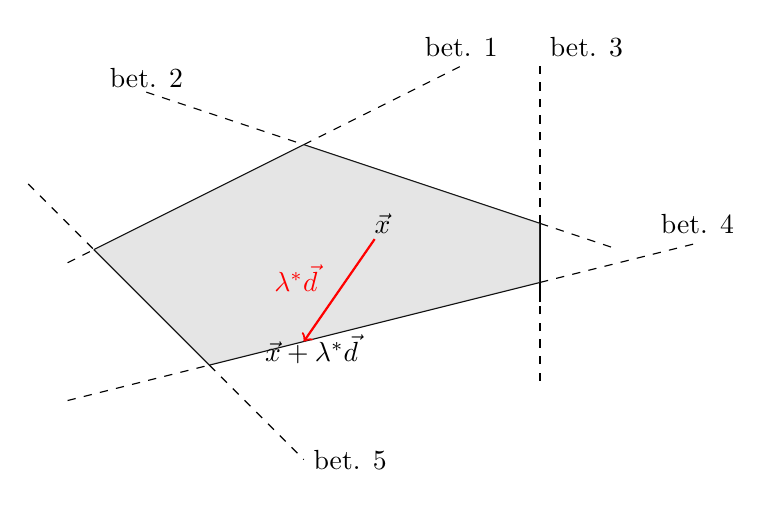
\begin{tikzpicture}[ latex
  s/.style={width=0}]

  %ligning 1
	\draw[domain=-1:-2/3,variable=\x,dashed] 	plot({\x},{0.5*\x+1});
	\draw[domain=-2/3:2,variable=\x] 			plot({\x},{0.5*\x+1});
	\draw[domain=2:4,variable=\x,dashed] 	plot({\x},{0.5*\x+1}) node[above] {bet. 1};
	
  %ligning 2
  	\draw[domain=0:2,variable=\x,dashed] 	plot({\x},{-(1/3)*\x+8/3}) node[above] at (0,2.6) {bet. 2} ;
	\draw[domain=2:5,variable=\x] 			plot({\x},{-(1/3)*\x+8/3});
	\draw[domain=5:6,variable=\x,dashed] 	plot({\x},{-(1/3)*\x+8/3});
	

  %ligning 3
  	\draw[domain=-1:0,variable=\y,dashed] 	plot({5},{\y});
	\draw[domain=0:1,variable=\y] 			plot({5},{\y});
	\draw[domain=1:3,variable=\y,dashed] 	plot({5},{\y}) node[above right] {bet. 3};
	
  %ligning 4
	\draw[domain=-1:4/5,variable=\x,dashed] 	plot({\x},{0.25*\x-1});
	\draw[domain=4/5:5,variable=\x] 			plot({\x},{0.25*\x-1});
	\draw[domain=5:7,variable=\x,dashed] 	plot({\x},{0.25*\x-1}) node[above] {bet. 4};
	
  %ligning 5
  	\draw[domain=-1.5:-2/3,variable=\x,dashed] 	plot({\x},{-\x}) ;
	\draw[domain=-2/3:4/5,variable=\x] 			plot({\x},{-\x});
	\draw[domain=4/5:2,variable=\x,dashed] 	plot({\x},{-\x}) node[right] {bet. 5} ;

  %løsningsmængden skraveret
	\fill[gray!80,nearly transparent] (4/5,-4/5) -- (-2/3,2/3) -- (2,2) -- (5,1) --(5,0.25) --  cycle;
	
  % vektor x
	\node[] (x) at (3,1) {$\vec{x}$};
	\draw[thick, color=red, ->](2.9,0.8) -- (2,-0.5) node[above, yshift=0.5 cm, xshift=-0.1 cm] {$\lambda^* \vec{d}$} ;
	\node[] (x) at (2.1, -0.6) {$\vec{x}+\lambda^* \vec{d}$};
 
\end{tikzpicture}
	\captionof{figure}{Der ligges et multiplum af en retnings vektor til vektor $\vec{x}$ til at summen gør betingelse $4$ aktiv.}
	\label{fig:eksistens}
\end{center}
\end{figure}
Det betyder at hvis det lineære programmerings problem er konsistent, da eksistere der enten en optimal løsning, blandt basisløsningerne eller den optimale løsning er $\pm \infty$.
Det kunne derfor være relevant at finde en måde, hvor den optimale løsning blandt basisløsningerne kan findes, her kan gøres brug af simplex metoden.




\chapter{Simplex} \label{afsnit:simplex}
En metode der kan bruges til at løse lineære programmerings problemer er simplex metoden. Kort fortalt går simplex metoden ud på at finde et punkt der opfylder alle givne uligheder, dette punkt findes i skæringpunktet mellem nogle funktioner for de givne uligheder. Herefter undersøges, i hvilken retning objektfunktionen vokser mest, og der fortsættes så i denne retning til et nyt punkt findes, hvor den retning der giver den største vækst igen findes. Dette gentages intil der ikke længere kan findes en retning hvor objektfunktionen vokser, og denne derfor må være optimal. 

I simplex metoden, bruges variable kaldet restvariable. Disse variable tilføjes til ligninger der beskriver uligheder, for at gøre dem til ligheder. 
\begin{defn}[Restvariable]
En restvariabel er en variabel, der tilføjes på den mindste side af en ulighed for at skabe en lighed. 
\end{defn}

Herunder ses et eksempel på hvordan en ulighed kan ændres til en lighed ved tilføjelse af restvariable.

\begin{eks}
Et lineært ligningssystem er givet,
\begin{align*}
5 x_1 + 2 x_2 &+ 2x_3 \leq 20 \\
3 x_1 + 4 x_2 &+ 3 x_3 \leq 30 \\
x_2 &+ 2 x_3 \leq 10.
\end{align*}
Nu tilføjes restvariable for at gøre de tre uligheder til ligheder,
\begin{align*}
5 x_1 + 2 x_2 &+ 2x_3 + x_4& &&\leq 20 \\
3 x_1 + 4 x_2 &+ 3 x_3 &+ x_5& &\leq 30 \\
x_2 &+ 2 x_3 & &+x_6 &\leq 10.
\end{align*}

\end{eks}
Hvis et lineært programmeirngproblem har en optimal mulig løsningen, så findes der en basis mulig løsning som er optimal. 
Simplex metoden søger efter denne optimale basis mulige løsning, ved at bevæge sig mellem de mulige basis løsninger. 
På et tidspunkt vil den optimale løsning være fundet, da der kun er et endeligt antal basis mulige løsninger. 
Denne søgen efter den optimale basis løsning kan gøres ved hjælp af forskellige typer Simplex. 
Nogen af disse vil blive gennemgået i dette kapitel. 

\section{kommer senere}
De algoritmer som bruges til at løse dette problem er ofte struktureret således at de med udgangspunkt en allerede kendte basis mulig løsning. Hvorefter der søges efter en bedere løsning i nærheden. 

Betragt en basis mulig løsning $\vec{x} \in P$. 
Det ønskes at rykke til en anden mulig løsning, dette gøres i rettingen af en vektor $\vec{d} \in \mathds{R}^n$. Det giver ikke mening at betragte de vektorer som med det samme kommer udenfor polyhedronet, $P$. Det er derfor kun de mulige retninger som betrages. 

\begin{defn}[Mulig retning]
Lad $\vec{x}$ være en vektor i $P$. En vektor $\vec{d}$ er en mulig retningen fra $\vec{x}$, hvis der findes en positiv scalar $\theta$ således at $\vec{x}+\theta\vec{d} \in P$ 
\end{defn}

Da polyhedronet er en konveks mængnde må det gælde at, hvis $\vec{x} \in P$ og $\vec{d}$ er en mulig retning, så er $\vec{x}+ \theta^{*} \vec{d} \in P$ for $\theta^{*} \in ] 0,\theta ] $

\section{Store M-metode}

For at kunne bruge simplex metoden, skal der først findes en mulig basis løsning. 
Hvis der er givet et problem på formen $Ax \leq b$, hvor $b \geq 0$ er det relativt simpelt. 
Her kan introduceres ikke-negative slack-variable $s$ og uligheden kan omskrives til $Ax+s=b$. 
Vektoren $(x,s)$ hvor $x=0$ og $s=b$ er en mulig basis løsning, og den korresponderende basismatrix er dens identitet. 
<<<<<<< HEAD
Generelt er det dog ikke let at finde en mulig basis løsning, og det kræver en løsning til et hjælpende lineært programmeringsproblem. \\
=======
Generelt er det dog ikke let at finde en mulig basis løsning, og det kræver at løsning til et hjælpende lineært programmeringsproblem. \\
>>>>>>> master

Store-M metoden bygger på den to-fase simplex metode, som er en komplet algoritme til at løse lineære programmeringsproblemer på standardform. 
Algoritmen er bygget op i to faser, hvor første fase går ud på .... \\
%?? skal det med

Idéen bag store-M metoden er at introducere en kostfunktion på formen
\begin{align*}
\sum\limits_{j=1}^n c_jx_j + M \sum\limits_{i=1}^m y_i,
\end{align*}
hvor $M$ er en stor positiv konstant, og $y_i$ er samme variable som i den første fase af to-fase simplex. 
Hvis det originale problem har en mulig løsning, og dens optimale kost er endelig, vil de artificial (kunstige?) variable gå mod $0$, når $M$ er tilstrækkelig stor. 
Det betyder, at den originale kostfunktion nu skal minimeres. 
Når den reducerede kost er en funktion af $M$, vil $M$ altid blive behandlet som værende af større værdi, når der skal vurderes, om en reduceret kost er negativ. \\

\begin{eks}
Et lineært programmeringsproblem er givet.

	\begin{center}
	\begin{tabular}{l >{$}r<{$}	>{$}r<{$} >{$}l<{$} >{$}l<{$} r}
	Minimer 		& 	x_1	 & + \ \ x_2 & + \ \ x_3 \\
	med hensyn til 	&  	x_1	 & +   2 x_2 & +   3 x_3 &  	 & = 3 \\
					&  -x_1	 & +   2 x_2 & +   6 x_3 & 		 & = 2 \\
					&  \ \ 	 & \ \ 4 x_2 & +   9 x_3 & 		 & = 5 \\
					&  \ \ 	 & \ \   	 & \ \ 3 x_3 & + x_4 & = 1 \\
	og $x_1, \dots, x_4 \geq 0$.
	\end{tabular}
	\end{center}

Der gives nu følgende problem til hjælp, hvor den unødvendige kunstige variabel $x_8$ er undladt.

	\begin{center}
	\begin{tabular}{l >{$}r<{$}	>{$}r<{$} >{$}l<{$} >{$}r<{$} >{$}r<{$} >{$}r<{$} >{$}r<{$} r}
	Minimer 		&  	x_1	 & + \ \ x_2 & + \ \ x_3 &       & + Mx_5    & + Mx_6    & + Mx_7 \\
	med hensyn til 	&  	x_1	 & +   2 x_2 & +   3 x_3 &       & + \ \ x_5 &           &        & = 3 \\
					&  -x_1	 & +   2 x_2 & +   6 x_3 &       &           & + \ \ x_6 &        & = 2 \\
					&        &     4 x_2 & +   9 x_3 &       &           &           & + \ \ x_7 & = 5 \\
					&   	 &           &     3 x_3 & + x_4 &           &           &       & = 1 \\
	og $x_1, \dots, x_7 \geq 0$.
	\end{tabular}
	\end{center}

%eks ikke færdigt. + tabellerne skal fikses
\end{eks}

hello world!

\chapter{Simplex Metoden}
Af forrige kapitel fremgik det, at den optimale løsning altid vil være en mulig basisløsning, og af Sætning \ref{stn:kravtilbasis}
fremgår det, hvordan en basisløsning findes. 
Problemet er, at hvis alle basisløsninger skal testes for et standard problem med uligheder, skal optil $\binom{n}{m}$ muligheder testes. 
Derfor er det nødvendigt, at finde en metode, hvorpå den optimale løsning kan findes uden at skulle kigge på hvert enkelt tilfælde. 
En af metoderne, som kan anvendes, er Simplex metoden. I dette kapitel vil Simplex metoden, og forskellige implementeringer af metoden, derfor blive gennemgået med udgangspunkt i .
\section{Udledning af Simplex metoden}
Simplex metoden starter med en basisløsning, og går så i en mulig retning indtil den finder en ny basisløsning.
\begin{defn}[Mulig retning]
%Lad $\vec{x} \in P$. En vektor $\vec{d}$ er en \textbf{mulig retningen} fra $\vec{x}$, hvis der eksistere en positiv skalar $\theta > 0$ således at $\vec{x}+\theta\vec{d} \in P$ 
%\end{defn}
Det er derfor nødvendigt at kunne skrive en basisløsning som et udtryk af en anden basisløsning og en mulig retningsvektor.
\begin{stn}
Lad $\vec{x} \in P =\{\vec{x}\in \mathds{R}^n \mid A\vec{x}= \vec{b}, \vec{x}\geq \vec{0}\}$ være en basisløsning. Da eksisterer der en vektor $\vec{d}\in \mathds{R}^n$, og en skalar $\theta^*\geq 0$ så $\vec{y}= \vec{x} + \theta^* \vec{d}$ er en basisløsning til $\vec{x}$, hvis $P$ ikke indeholder en linje.
\label{stn:matbagsim}
\end{stn}
Sætning \ref{stn:matbagsim} består af tre påstande; at der eksisterer en vektor $\vec{d}$, en skalar $\theta^*$ og at $\vec{y}$ er en basisløsning.
Derfor splittes sætningen op i lemmaer, og eksistensen af $\vec{d}$ vises først.
\begin{lma}
Lad $\vec{x} \in P =\{\vec{x}\in \mathds{R}^n \mid A\vec{x}= \vec{b}, \vec{x}\geq \vec{0}\}$ være en basisløsning. Da eksisterer der en vektor $\vec{d}\in \mathds{R}^n$, så $\vec{x} + \vec{d} \in P$, og så $\vec{d}$ introducerer $x_j$ og kun $x_j$ til basisløsningen.
\label{lma:retningsvektor}
\end{lma}
\begin{proof}
%Først konstrueres $\vec{d}$.
Lad $B$ betegne basismatricen til $\vec{x}$, så $\vec{A_{B(i)}}$ er en søjle i $B$ for et index $I_B =\{B(1),...,B(m)\}$. 
%Da $\vec{y}$ skal være en nabo basisløsning, må der eksistere en variable $x_j$ for $j \notin I_B$, så $x_j = 0$ for $\vec{x}$ og $\vec{x_j} \neq 0 $ for $\vec{y}$. 
Da skal $\vec{d}$ introducere $x_j$ og kun $x_j$ til basisløsningen, konstruer derfor $\vec{d}$ så $x_j \neq 0$ for $\vec{x}+\vec{d}$, lad derfor $d_j=1$, og $d_i = 0$ for $i\notin I_B$ og $i \neq j$. 
Bemærk at da $\vec{x}+ \theta^*\vec{d} \in P$ må
\begin{align*}
	A(\vec{x}+\theta^* \vec{d}) = A\vec{x} + \theta^* A \vec{d}  & = \vec{b} \qquad \Rightarrow
	\\ A \vec{d} &= \vec{0}
\end{align*}
Lad nu $\vec{d}_B$ betegne indgangene i $\vec{d}$ så $d_i \in \vec{d}_B$ for $i \in I_B$. 
Det følger derfor, at
\begin{align*}
A \vec{d} = \sum_{i \in I_B} \vec{A_i} \vec{d_i} + \vec{A_j} &= B\vec{d}_B + \vec{A_j} = 0 \qquad \Rightarrow
\\ \vec{d}_B &= -B^{-1}\vec{A_j}.
\end{align*}
Bemærk, at $B^{-1}$ eksistere ifølge Sætning %Mangler.
Det betyder at $\vec{d}_B = -B^{-1}\vec{A_j}$, mens at $d_j = 1$ og $d_i = 0$ for $i\notin I_B$ og $i \neq j$.
\end{proof}
Det fremgår af beviset for Lemma \ref{lma:retningsvektor} at $\vec{d}$ eksisterer og kan skrives som et udtryk af basismatricen til $\vec{x}$ og den $j$ søjle i $A$. 
Vektoren $\vec{d}$ defineres derfor som den $j$te retningsvektor. 
\begin{defn}[$j$te retningsvektor]
Lad $\vec{x} \in P =\{\vec{x}\in \mathds{R}^n \mid A\vec{x}= \vec{b}, \vec{x}\geq \vec{0}\}$ være en basisløsning med basis matrix $B$, så $\vec{A_{B(i)}}$ er en søjle i $B$ for et index $I_B =\{B(1),...,B(m)\}$, da er den \textbf{$j$te retningsvektor} givet ved $\vec{d}_B = - B^{-1} A_j$ $d_j = 1$ og $d_i = 0$ for $i\notin I_B$ og $i \neq j$.
\end{defn}
For at $\vec{y}$ kan være en basisløsning må den kun have $m$ basis variable, og da $\vec{d}$ introducere en ny variabel til løsningen, må $\theta^*$ skulle konstrueres så den fjerner en variable fra løsningen.
\begin{lma}
Lad $\vec{x} \in P =\{\vec{x}\in \mathds{R}^n \mid A\vec{x}= \vec{b}, \vec{x}\geq \vec{0}\}$ være en basisløsning, og $\vec{d}$ være den $j$te retningsvektor.
Da eksisterer en skalar $\theta^* \geq 0$, så $\vec{x} + \theta^* \vec{d} \in P$, og så $\theta^* $ fjerner $x_l$ fra basisløsningen, hvis $P$ ikke indeholder en halvlinje.
\label{lma:skalar}
\end{lma}
\begin{proof}
Lad $B$ betegne basismatricen til $\vec{x}$, så $\vec{A_{B(i)}}$ er en søjle i $B$ for et index $I_B =\{B(1),...,B(m)\}$. 
Antag først, at $\vec{d}\geq \vec{0}$, da vil $\vec{x}+\theta^*\vec{d}$ altid overholde alle lighedsbetingelser og positivitetsbetingelser for $\theta^* \geq 0$. 
Derfor vil $P$ indeholde en linje, da det går mod antagelsen om at $P$ ikke indeholder en linje, må mindst en indgang i $\vec{d}$ være negativ, kald denne for $d_i$.
Da må 
\begin{align*}
 0 &= x_i + \theta^* d_i \qquad \Rightarrow
 \\ \theta^* = -\frac{d_i}{x_i}.
\end{align*} 
\\Hvis $\vec{x} + \theta^* \vec{d} \in P$, må intet $x_i$ blive mindre end $0$, hvorfor $x_l$ vælges så $\frac{x_i}{d_i}$ er så lille som muligt for $d_i < 0$. 
Dermed bliver $\theta^* = \underset{i \in I_B}{\min}\{\frac{x_i}{d_i}\}$. 
\end{proof}
Bemærk at da det er antaget at ingen løsninger er degenrete, følger det af Sætning %Mangler
, at $\theta^*$ fjerner en og kun en basisvariable fra løsningen.
Igen kan $\theta$ defineres udfra formlen fundet i beviset for Lemma \ref{lma:skalar}.
\begin{defn}[$j$te skalar]
Lad $\vec{x} \in P =\{\vec{x}\in \mathds{R}^n \mid A\vec{x}= \vec{b}, \vec{x}\geq \vec{0}\}$ være en basisløsning, $\vec{d}$ være den $j$te retningsvektor, og $P$ ikke indeholder en linje.
Da er den \textbf{$j$te skalar} givet ved $\theta^* = \underset{i \in I_B}{\min}\{\frac{x_i}{d_i}\}$.
\end{defn}
Efter at have vist både eksistensen af $\vec{d}$ og skalaren $\theta^*$, kan det vises at $\vec{y}$ er en basisløsning. 
Sætning \ref{stn:matbagsim} bevises derfor.
\begin{proof}
Det følger af Lemma \ref{lma:retningsvektor} og Lemma \ref{lma:skalar}, at $\vec{d}$ og $\theta^*$ eksistere. 
For at vise at $\vec{y}$ er en basisløsning, bemærkes at $x_i = 0$ for $i \notin I_{B'} = I_B\setminus\{l\}\cup\{j\}$ og at Basismatricen for $\vec{y}$ er matricen $B'$ med søjlerne $A_i$ for $i \in I_{B'}$. 
Det følger derfor af Sætning \ref{stn:kravtilbasis},
at $\vec{y}$ er en basisløsning, hvis søjlerne i $B'$ er lineært uafhængige.
Antag derfor for modstrid, at søjlerne er lineært afhængige, da følger det af Definition \ref{defn_lin_uafh},
at
\begin{align*}
 \sum_{i \in I_{B'}} \lambda_i A_i = \vec{0}.
\end{align*}
Da $B$ og $B'$ kun er forskellige i en søjle, må
\begin{align*}
 \\ \sum_{i \in I_{B'}}  B^{-1} \lambda_i A_i  =\sum_{i \in I_{B'}\setminus \{j\}} \vec{e_i} + B^{-1} \lambda_j A_j = \vec{0}.
\end{align*}
Dvs. at søjlerne i $B'$ er lineært uafhængige, hvis $A_{jl} = 0$.
Bemærk at $B^{-1} \lambda_j A_j = - \vec{d}_B$, hvis $l$te indgang pr. definition er forskellig fra $0$. 
Alle søjler i $B'$ er altså lineært uafhængige, hvorfor alle rækker er lineært uafhængige og $\vec{y}$ er en basisløsning.
Bemærk, at da $\vec{x}\in P$ og $\vec{d}$ og $\theta^*$ er konstrueret så $\vec{x}+\theta^*\vec{d} \in P$ må $\vec{y} \in P$, hvormed $\vec{y}$ er en mulig basisløsning.
\end{proof}
Det er nu vist, hvordan det er muligt at gå fra en basis løsning til en anden.
 Bemærk at de to løsninger er naboløsninger, da det er antaget at ingen af dem er degenerate, og der derfor kun bliver introduceret en ny variable og fjernet en gammel, hvorfor at løsningerne må dele samme krav på nær et. 
Det er nu nødvendigt at finde en måde, så at den basisløsning, som findes minimere objektfunktionen mere end den foregående, ellers vil alle basisløsninger stadig skulle tjekkes. 
\begin{stn}
Lad $\vec{x}$ være en basisløsning, med basismatrix $B$, da er ændringen i obejktfunktionen ved at introducere $x_j$ til løsningen givet ved
\begin{align*}
 \Delta c_j = c_j-\vec{c}_B B^{-1}\vec{A_j}.
\end{align*}
\label{stn:Deltac}
\end{stn}
\begin{proof}
Antag først at $x_j$ ikke er en basis variable til at starte med, da vil den $j$te retningsvektor introducere $x_j$ til løsningen, hvorfor,
\begin{align*}
\Delta c_j = \vec{c}^T(\vec{x}+ \vec{d}) - \vec{c}^T\vec{x} = \vec{c}^T\vec{d} = \sum_{i \in I_B} c_i d_i + c_j.
\end{align*}
Lad nu $\vec{c}_B = \rvect{c_{B(1)}& \cdots & c_{B(m)}}$, da vil
\begin{align}
\Delta c_j =\vec{c}_B\vec{d}_B+ c_j = c_j-\vec{c}_B B^{-1}\vec{A_j}.
\end{align}
Antag nu at $x_j$ er en basisvariable da vil 
\begin{align*}
\Delta c_j = \vec{c}^T\vec{x}- \vec{c}^T\vec{x} = 0.
\end{align*}
Det undersøges derfor om $ c_j-\vec{c}_B B^{-1}\vec{A_j}= 0$, hvis $x_j$ er en basisvariable.
\begin{align*}
 \Delta c_j = c_j-\vec{c}_B^T B^{-1}\vec{A_j} = c_j - \vec{c}_B^T \vec{e_j} = c_j - c_j = 0.
\end{align*}
Det kan derfor konkluderes at $\Delta c_j = c_j-\vec{c}_B B^{-1}\vec{A_j}$ for et hvert $x$.
\end{proof}
Det må derfor være bedst at gå enten i den retning hvor $\Delta c_j$ er størst eller $\theta^*\Delta c_j$ er størst. 
Hvis der ikke sker en ændring eller ændringen forstørrer objektfunktionen må den fundne basisløsning nødvendigvis være optimal.
\begin{stn}
Lad $\vec{x}$ være en basisløsning, med basismatrix $B$, så er $\vec{x}$ optimal, hvis og kun hvis $\Delta c_j \geq 0$ for alle $j$.
\label{stn:optimalDeltaC}
\end{stn}.
\begin{proof}
Antag først at $\vec{x}$ er optimal, da vil $\vec{c}^T\vec{x} \leq \vec{c}^T\vec{y}$ for alle $\vec{y} \in P$. 
Antag for modstrid at $\Delta c_j < 0$ for en basisvariable $x_j$, da følger det at $\vec{c}^T(\vec{x}+\theta^*\vec{d}) = \vec{c}^T\vec{x} + \Delta c_j \leq \vec{c}^T\vec{x}$, hvilket strider mod antagelsen om at $\vec{x}$ er optimal.
Antag nu, at $\Delta c_j \geq 0$ og lad $\vec{y}$ være en vilkårlig vektor i $P$, og lad $\vec{d}=\vec{y}-\vec{x}$.
Bemærk at $A\vec{d} = A\vec{y}- A\vec{x} =  \vec{b} - \vec{b} =\vec{0}$.
Lad nu $\vec{d}_B = \rvect{d_{B(1)} & \cdots & d_{B(m)}}^T$, og lad $N= \{i \leq n| i \neq B(1),...,B(m)\}$, da kan matrix-vektorproduktet omskrives til:
\begin{align*}
	B\vec{d}_B + \sum_{i \in N} \vec{A}_i d_i = \vec{0} \qquad \Rightarrow
	\\ \vec{d}_B = - B^{-1}\sum_{i \in N} \vec{A}_i d_i
\end{align*}
Bemærk at det benyttes at $B$ er invertibel ifølge Sætning %Mangler
Da tages objektfunktionen til $\vec{d}$ for at finde prisen for at gå fra $\vec{x}$ til $\vec{y}$.
\begin{align*}
 \vec{c}^T\vec{d} &= \vec{c}_B^T\vec{d}_B + \sum_{i \in N} c_i d_i 
 \\&= \vec{c}_B^T(- B^{-1}\sum_{i \in N} \vec{A}_i d_i) + \sum_{i \in N} c_i d_i  
 \\&= \sum_{i \in N} (- \vec{c}_B^T B^{-1} \vec{A}_i d_i) +  c_i d_i 
 \\&= \sum_{i \in N} ( c_i - \vec{c}_B^TB^{-1}\vec{A}_i ) d_i
\end{align*}
Det følger af Sætning \ref{stn:Deltac} at $\Delta c_i = c_i - \vec{c}_B^TB^{-1}\vec{A}_i $, hvorfor
\begin{align*}
\vec{c}^T\vec{d} = \sum_{i \in N} \Delta c_i d_i.
\end{align*}
Da $\vec{x}$ er en basisløsning må $x_i = 0$ for $i \in N$, og da $\vec{y} \in P$ må $\vec{y} \geq \vec{0}$, dermed må $d_i = y_i - x_i \geq 0$, og da $\Delta c_i$ var antaget at være ikke negativ, medfører det at
\begin{align*}
\vec{c}^T\vec{d} = \vec{c}^T\vec{y}-\vec{c}^T\vec{x} \geq 0 \qquad \Rightarrow
\\ \vec{c}^T\vec{x} \leq \vec{c}^T\vec{y}
\end{align*}
for et hvert $\vec{y} \in P$, da $\vec{y}$ var vilkårligt valgt, derfor må $\vec{x}$ være optimal.
\end{proof}
Det kan alt sammen opsummeres til Simplex metoden

\begin{pro}[label=pro:simplex,style=ingental]{Procedure for Simplex metoden}
1. Vælg en basisløsning $\vec{x}$ med basismatrix $B$
2. Beregn $\Delta c_j$ for alle $j \notin I_B$. 
   Hvis $\Delta c_j\geq 0$ for alle $j \notin I_B$ 
   	   stop, $\vec{x}$ er optimal.
   Hvis $\Delta c_j < 0$ for en $j \notin I_B$
       vælg mindste $c_j$.
3. Find $\vec{d}_j$
   Hvis $d_i \geq 0 $ for alle $i \in I_B$ 
       stop, den optimaleværdi er $- \infty$.
   Hvis $d_i < 0 $ for mindst et $i \in I_B$ 
       vælg $B(l)$ så $\frac{x_{B(l)}}{d_{B(l)}}\leq \frac{x_i}{d_i} $ for ethvert $i \in I_B$
4. Find $\theta^*$
5. Find den nye basisvektor og basismatrix.
6. Gå til step 2.
\end{pro}

Til sidst vises at Simplex metoden altid vil finde frem til den optimale løsning efter et endeligt antal interationer.
\begin{stn}
Lad $P \neq \emptyset$, da stopper Simplex metoden efter et endeligt antal interationer, enten ved at finde den optimale løsning eller at den optimale værdi er $- \infty$.
\end{stn}
\begin{proof}
Antag først at Simplex metoden stopper efter step 2 i Program \ref{pro:simplex}, da følger det af Sætning \ref{stn:optimalDeltaC}
at basisløsningen er optimal, og Simplex metoden har derfor fundet den optimale løsning.
\\ Antag nu at Simplex metoden stopper efter step 3 i Program \ref{pro:simplex}, da følger det af beviset for Lemma \ref{lma:skalar}, at $P$ indeholder en linje, hvorfor det følger af Afsnit \ref{sec:eksistens},
at den optimale værdi er $-\infty$.
\\ Da der kun er en endelig mængde basisløsninger i følge Korollar \ref{kor:endeligbasis}
må Simplex metoden altid stoppe, med mindre, at den cirkulere igennem de samme basisløsninger.
Da den $j$te retningsvektor altid vælges så $\Delta c_j < 0$, må den samme basisløsning aldrig kunne blive besøgt mere end en gang, hvorfor der ikke kan opstå en ring, og Simplex metoden må derfor stoppe efter et endeligt antal interationer.
\end{proof} 





\chapter{Case}
Teorien omkring Store-M metoden vil nu blive anvendt til optimeringen af en specifik case. Problemet, som skal optimeres, er tildelingen af arbejdsopgaver til ansatte i en virksomhed. 
I denne case adskiller de ansatte sig fra hinanden i forhold til både løn, maksimalt antal arbejdstimer, samt deres effektivitet i løsningen af de forskellige opgaver. 
Yderligere skal hver opgave løses et bestemt antal gange.
Optimeringsproblemet går, med udgangspunkt i disse betingelser, ud på at minimere firmaets udgifter til løn. Netop Store-M metoden anvendes, da problemet ikke har en åbenlys basisløsning, og det kan derfor løses med et enkelt optimeringsproblem.\\

Lad en virksomhed have $G$ ansatte, hvor den $i$'te ansatte maksimalt må arbejde $T_i$ timer, hvor $i=1, \dots, G$. Virksomheden har $H$ arbejdsopgaver, som hver skal løses $O_j$ gange, hvor $j=1, \dots, H$.
Her gælder det, at $p_{ij}$ er den mængde tid, den $i$'te ansatte bruger på den $j$'te opgave med en effektivitet på $n_{ij}$. Derudover har hver ansat en individuel løn $L_i$.
Disse oplysninger er samlet i følgende programmeringsproblem, som søger at minimere udgifterne:

\begin{center}
	\begin{tabular}{l	>{$}l<{$}}
Minimer			&\sum_{i=1}^G L_i \left( \sum_{j=1}^H p_{ij} \right)\\
\rule{0pt}{4ex}Med hensyn til 	&T_i \geq \sum_{j=1}^H p_{ij},\\
				&O_{j} = \sum_{i=1}^G n_{ij} p_{ij}\\
og $p_{ij} \geq 0.$
	\end{tabular}
\end{center}

Derved består det nødvendige input af vektorer $\vec{L}$, $\vec{T}$ og $\vec{O}$, for henholdsvis løn, timetal og opgavekrav. Matricen $N$ viser de ansattes effektiviteter til de forskellige opgaver:
\begin{align*}
	N=\kbordermatrix{
	Ansatte \backslash Opgaver & 1 & 2 & \dots & H\\
	1		&	n_{1,1}	&	n_{1,2}	&	\dots	&	n_{1,H}\\
	2		&	n_{2,1}	&	n_{2,2}	&	\dots	&	n_{2,H}\\
	\vdots	&	\vdots	&	\vdots	&		& 	\vdots\\
	G		&   n_{G,1}	&	n_{G,2}	&	\dots	&	n_{G,H}
	}
\end{align*}


Ved anvendelse af Store-M metoden til løsningen af dette problem, skal der anvendes slack-variable og kunstige variable. Enhver ulighed skal omskrives til en lighed, hvilket kræver indførslen af en slack-variabel. Da begrænsningerne for de ansattes timetal er mindreendbetingelser, kan disse omskrives til:
$$T_i = \sum_{j=1}^H p_{ij}+s_i$$
I Store-M metoden kræver denne begrænsning ikke en ekstra variabel med cost $M$, da $s_i$ gerne må være over $0$ i den endelige løsning.

Begrænsninger af typen
$O_{j} = \sum_{i=1}^G n_{ij} p_{ij},$
kræver en ekstra variabel $a_j$ med cost $M$ for at kunne danne en begyndende basisløsning. Derved omskrives disse begrænsninger til
$O_{j} = \sum_{i=1}^G n_{ij} p_{ij}+a_j$.
Variablene $a_j$ må ikke have en værdi over $0$ i den endelige basis, da de originale ligheder derved ikke overholdes. Derfor får disse variable en cost $M$, så de reduceres til $0$, hvis dette er muligt.

Derved kan problemet omskrives til:
\begin{center}
	\begin{tabular}{l	>{$}l<{$}}
Minimer			&\sum_{i=1}^G L_i \left( \sum_{j=1}^H p_{ij} \right)+M\sum_{j=1}^H a_j\\
\rule{0pt}{4ex}Med hensyn til 	&T_i = \sum_{j=1}^H p_{ij} + s_i\\
				&O_{j} = \sum_{i=1}^G n_{ij} p_{ij}+a_j\\
og $p_{ij} \geq 0.$
	\end{tabular}
\end{center}

Der vil derved være $G \cdot H$ variable, $p_{ij}$, $G$ slack-variable, $s_i$, og $H$ kunstige variable, $a_j$. Dette giver i alt $G \cdot H+G+H$ variable i $G+H$ betingelser. 

\section{Konstruktion af simplex tabellen for casen}
Ved konstruktionen af den fulde tabel tilføjes endnu en række og søjle. Derved får tabellen størrelsen $(G+H+1) \times (G\cdot H+G+H+1)$. 
Løsningsvektoren og cost-vektoren bliver derved:

\begin{align*}
\vec{x}^T &= \ \ \rvect{p_{11} ... p_{1H} & ... & p_{G1} ... p_{GH} & s_1 ... s_G & a_1 ... a_H},\\
\vec{c}^T &=\kbordermatrix{
& \times H & & \times H & \times G & \times H \\
&L_1 & ... & L_G & 0 & M
},
\end{align*}
hvor f.eks. $\times H$ betyder, at denne indgang udgør $H$ indgange af vektoren.

Ved introduktionen af slack-variable og kunstige variable, kan disse derved udgøre den første basis for ligningssystemet. Derved bliver basisindekset og basisvektoren til:
\begin{align*}
&\vec{I}_B^T=\rvect{s_1 ... s_G & a_1 ... a_H},\\
&\vec{x}_B^T=\rvect{T_1 ... T_G & O_1 ... O_H},
\end{align*}
da $p_{ij}=0$ for $i=1,2,...,G$ og $j=1,2,...,H$. Leddene $s_i$ og $a_j$ er derved de eneste ikke-nul led i betingelserne.


Betingelserne kan da indskrives i matricen $A$. For et problem med $G=2$ og $H=3$ gælder det derved, at
\begin{align*}
B^{-1}A=\kbordermatrix{
&p_{11} & p_{12} & p_{13} & p_{21} & p_{22} & p_{23} & s_1 & s_2 & a_1 & a_2 & a_3\\
&1       & 1      & 1      & 0      & 0      & 0      & 1 & 0 & 0 & 0 & 0 \\
&0       & 0      & 0      & 1      & 1      & 1      & 0 & 1 & 0 & 0 & 0 \\
&n_{11}  & 0      & 0      & n_{21} & 0      & 0      & 0 & 0 & 1 & 0 & 0 \\
&0       & n_{12} & 0      & 0      & n_{22} & 0      & 0 & 0 & 0 & 1 & 0 \\
&0       & 0      & n_{13} & 0      & 0      & n_{23} & 0 & 0 & 0 & 0 & 1
}_,
\end{align*}
da $B^{-1}=B=I_{G+H}$. Det gælder derfor, at $B^{-1}A=I_{G+H}A=A$.\\

Den reducerede cost for en ændring af $x_j$ er givet som $\Delta c_j=\vec{c}_j-\vec{c}_BB^{-1}\vec{A}_j.$

For denne case og opstilling af $B^{-1}A$ er det muligt at simplificere denne udregning.

Variablen $p_{ij}$ har i $A$ og $\vec{c}$ et indeks $k=(i-1)\cdot H+j$. Den reducerede cost for en sådan variabel kan findes som:
\begin{align*}
	\Delta c_{k} \ &=  \vec{c}_{k}-\vec{c}_B B^{-1}\vec{A}_{k}\\
	&= \ L_i-\vec{c}_B \vec{A}_{k} \\
	&= \ L_i-M \cdot n_{ij},
\end{align*}
da søjlevektoren for en given variabel $p_{ij}$ kun har 2 ikke-nul indgange, hvoraf den korresponderende cost for den ene af dem er lig $0$.

Derved bliver den reducerede cost-vektor til:
\begin{align*}
\bar{c}=	& \kbordermatrix{
& & & & \times (G+H)\\
&L_1-Mn_{11} \ \dots \ L_1-Mn_{1H} & \dots & L_G-Mn_{G1} \ \dots \  L_G-Mn_{GH} & 0}
\end{align*}

Den første simplex-tabel kan hermed, for et problem med $G=2$ og $H=3$, opskrives som:\\

\scalebox{0.8}{
\begin{tabular}{| >{$}l<{$} | >{$}l<{$}>{$}l<{$}>{$}l<{$}>{$}l<{$}>{$}l<{$}>{$}l<{$}>{$}l<{$}>{$}l<{$}>{$}l<{$}>{$}l<{$}>{$}l<{$} |}
\hline
-(O_1+O_2+O_3)M	&L_1-Mn_{11} &L_1-Mn_{12} &L_1-Mn_{13} &L_2-Mn_{21} &L_2-Mn_{22} &L_1-Mn_{23} &0 &0 &0 &0 &0\\
\hline
T_1	&1       & 1      & 1      & 0      & 0      & 0      & 1 & 0 & 0 & 0 & 0 \\
T_2 &0       & 0      & 0      & 1      & 1      & 1      & 0 & 1 & 0 & 0 & 0 \\
O_1	&n_{11}  & 0      & 0      & n_{21} & 0      & 0      & 0 & 0 & 1 & 0 & 0 \\
O_2	&0       & n_{12} & 0      & 0      & n_{22} & 0      & 0 & 0 & 0 & 1 & 0 \\
O_3 &0       & 0      & n_{13} & 0      & 0      & n_{23} & 0 & 0 & 0 & 0 & 1\\
\hline
\end{tabular}
}


\section{Løsning af problemet}
For at løse optimeringsproblemet dannes den fulde tabel ligesom i Fuld tabel metoden, hvorfor den også kan løses på samme måde.
For netop denne case er der nogle faktorer, som betyder, at problemet bliver simplificeret.
Da alle indgange i $B^{-1}$ og $\vec{x}_B$ er positive, vil alle rækker, ifølge Sætning \ref{stn:lexi}, forblive leksikografisk positive, hvorved der ikke er behov for at bytte om på søjlerne for at kunne anvende den leksikografiske pivotregel.
Da der findes en entydig variabel i hver betingelse, garanterer dette, at rækkerne er lineært uafhængige, hvorved de fundne basisløsninger nødvendigvis har dimension $0$. Derved er det ikke nødvendigt at tage højde for eventuelle tilfælde med lineært afhængige rækker. Da alle variable har en cost større end $0$, og da ingen af disse kan være negative, er det heller ikke muligt at opnå et tilfælde med uendeligt lav cost. Derved er det udelukkende nødvendigt at undersøge 2 scenarier: 
\begin{itemize}
\item Problemet har en optimal løsning.
\item Problemet har ingen løsning.
\end{itemize}


Til løsningen af problemer af denne type er der dannet følgende algoritmer med funktioner, som finder en optimal løsning. Algoritme \ref{alg:lexi} finder den leksikografisk mindste række i tabellen, for de rækker, som har en indgang over nul i pivotsøjlen. 

Algoritme \ref{alg:storem2} er den overordnede algoritme, som laver nye iterationer, indtil en optimal løsning er fundet. Yderligere defineres to konstanter $m$ og $n$, som er henholdsvis højde og bredde af den fulde tabel. Her gælder det i algoritmerne, at matricen $A$ er den fulde tabel.

\newpage

\begin{alg}[label={alg:storem2}]{Store-M algoritmen}
def $\textbf{storeM}$(A,I_B):
    mens sandt: #kører iterationer indtil løsning fundet
    	piv_søjle = 0
    	for søjle i range(1,n-1): 
        	hvis A[0][søjle] < 0: # finder søjle med ${\color{commentgreen} \overline{c}_i}$<0
            	piv_søjle = søjle
            	break
		hvis piv_søjle = 0: #hvis ingen reduceret cost er negative så afsluttes
			break
            
    	piv_række=$\textbf{lexi}$(A,piv_søjle) #finder den lexi-mindste række
            
    	piv_punkt = A[piv_række][piv_søjle] 
    	for søjle i range(n): #dividerer piv række med piv punkt
        	A[piv_række][søjle] /= piv_punkt
            
    	for række i range(m): #trækker piv række fra andre rækker
        	hvis række != piv_række:
            	række_trækfra = A[række][piv_søjle]
            	for søjle i range(n):
                	A[række][søjle] -= række_trækfra*A[piv_række][søjle]

    	I_B[piv_række-1]=piv_søjle #ny variabel indsættes i indeks for basis

	for indeks i $I_B$: 
		hvis indeks > G*H+G: #kunstig variabel stadig i basis. 
			hvis A[indeks+1][0] > 0: #kunstig variabel større end 0 giver uendeligt stor cost
				returner cost = $\infty$
	ellers: #løsning fundet
		returner cost = $-A[0][0]$
\end{alg}

\begin{alg}[label={alg:lexi}]{Leksikografisk pivot algoritme}
def $\textbf{lexi}$(A,piv_søjle):
	minrække = [række for række i $I_B$ for hvilke A[række][piv_søjle] > 0]
	
	for søjle i range(n):
		$\theta$ = [A[række][søjle]/A[række][piv_søjle] for række i minrække]
		minrække = [rækker i minrække for hvilke $\theta$[række] = min($\theta$)]
		hvis længde af minrække == 1:
			returner minrække[0] #række fundet og returneres
\end{alg}




\begin{eks}[Case eksempel]
Lad en virksomhed have $3$ medarbejdere, som skal have udført $4$ opgaver og lad parametrene være givet som:
\begin{align*}
\vec{L}=&	\rvect{120 & 200}\\
\vec{T}=&	\rvect{15 & 37}\\
\vec{O}=&	\rvect{200 & 60 & 70}\\
N=&\begin{bmatrix}
10	&2	&7\\
15	&3	&8\\
\end{bmatrix}
\end{align*}
Den fulde tabel, for dette problem, er derved følgende:\\

\scalebox{0.9}{
\begin{tabular}{| >{$}l<{$} | >{$}l<{$}>{$}l<{$}>{$}l<{$}>{$}l<{$}>{$}l<{$}>{$}l<{$}>{$}l<{$}>{$}l<{$}>{$}l<{$}>{$}l<{$}>{$}l<{$} |}
\hline
-330M	&120-10M &120-2M 	&120-7M	&200-15M &200-3M &200-8M & 0 & 0 & 0 & 0 & 0\\
\hline
15		&1		& 1    	& 1    	& 0      & 0     & 0     & 1 & 0 & 0 & 0 & 0\\
37 		&0  	& 0    	& 0     & 1      & 1     & 1     & 0 & 1 & 0 & 0 & 0\\
200		&10  	& 0    	& 0     & 15 	 & 0     & 0     & 0 & 0 & 1 & 0 & 0\\
60		&0  	& 2    	& 0     & 0      & 3 	 & 0     & 0 & 0 & 0 & 1 & 0\\
70 		&0  	& 0		& 7 	& 0      & 0     & 8 	 & 0 & 0 & 0 & 0 & 1\\
\hline
\end{tabular}
}\\

Ved anvendelse af Algoritme \ref{alg:storem2} findes følgende resultat for arbejdstiderne

\begin{align*}
P=\begin{bmatrix}
5 & 0 & 10\\
10 & 20 & 0
\end{bmatrix}
\end{align*}

Det ses, at denne løsning opfylder alle de originale betingelser:

\begin{center}
\begin{tabular}{>{$}l<{$}>{$}l<{$}>{$}l<{$}>{$}l<{$}>{$}l<{$}>{$}l<{$}>{$}l<{$}}
p_{11} 		& p_{12} 	& p_{13} 	& p_{21} 	& p_{22} 	& p_{23} 	&\\
1\cdot 5	& 1 \cdot 0	& 1\cdot 10	&			&			&			& \leq 15	\\
			&			&			&1\cdot 10 	&1\cdot 20	& 1\cdot 0	& \leq 37	\\
10\cdot 5 	&			&			&15\cdot 10 &			&			& =200	\\
			&2 \cdot 0	&			& 			&3\cdot 20	&			& =60	\\
			&			&7 \cdot 10	&			&			&8\cdot 0	& =70	\\
\end{tabular}
\end{center}

Dermed bliver den mindste løn, som skal udbetales, $15 \cdot 120 + 30 \cdot 200 = 7800$ kr.

\end{eks}

Ved at anvende denne algoritme er det nemt at optimere problemer med arbejdsfordeling, da dette giver en del forsimplinger i anvendelsen af Store-M metoden. 

% Appendicer indsættes inde i en appendices-blok og bliver nummereret med
% bogstaver i stedet for tal
\begin{appendices}
  % \include{incl/app/appendix1}
  % \include{incl/app/appendix2}
  % ..
\end{appendices}

% Dokumentets 'back matter' er til ekstra ting som f.eks. litteraturlisten.
% Overskrifter bliver ikke nummereret her.
\backmatter

% Automatisk litteraturliste baseret på, hvilke kilder, der er blevet refereret
% til i løbet af rapporten.
\bibliographystyle{apalike}
\bibliography{
  incl/bib/books,
  incl/bib/articles,
  incl/bib/software
}

\end{document}
